%% main_ppgco_ufu.tex v1.0, Lásaro Camargos e Denise Guliato
% adaptado de modeloABNT2.tex, v1.0 athila 
% ------------------------------------------------------------------------
% ------------------------------------------------------------------------
% eesc: Modelo de Trabalho Acadêmico (tese de doutorado, dissertação de
% mestrado e trabalhos monográficos em geral) em conformidade com 
% ABNT NBR 14724:2011. Esta classe estende as funcionalidades da classe
% abnTeX2 elaborada de forma a adequar os parâmetros exigidos pelas 
% normas USP e do departamento de elétrica da Escola de Engenharia 
% de São Carlos - USP.
% ------------------------------------------------------------------------
% ------------------------------------------------------------------------

% ------------------------------------------------------------------------
% Opções:
% 	tesedr:     Formata documento para tese de doutorado
%	qualidr:    Formata documento para qualificação de doutorado
% 	dissertmst: Formata documento para dissertação de mestrado
% 	qualimst:   Formata documento para qualificação de mestrado
% ------------------------------------------------------------------------
\documentclass[dissertmst]{ppgco}
%Não altere o comando seguinte. O título de seu trabalho será especificado mais adiante.
\title{Template de Monografia do PPGCO}

% ---
% PACOTES
% ---

% ---
% Pacotes fundamentais 
% ---
\usepackage{cmap}				% Mapear caracteres especiais no PDF
\usepackage{lmodern}				% Usa a fonte Latin Modern			
\usepackage{makeidx}            	% Cria o indice
\usepackage{hyperref}  			% Controla a formação do índice
\usepackage{lastpage}			% Usado pela Ficha catalográfica
\usepackage{indentfirst}			% Indenta o primeiro parágrafo de cada seção.
\usepackage{nomencl} 			% Lista de simbolos
\usepackage{graphicx}			% Inclusão de gráficos
\usepackage{multirow}
\usepackage{tabularx}
\usepackage{amsmath}
\usepackage[font=small]{caption}
% ---

% ---
% Pacotes adicionais, usados apenas no âmbito do Modelo eesc
% ---
\usepackage{lipsum}				       % para geração de dummy text
\usepackage[printonlyused]{acronym}
\usepackage[table]{xcolor}
\usepackage{longtable}

% ---
\makeatletter
\setlength{\@fptop}{0pt}
\makeatother

% ---
% Informações de dados para CAPA e FOLHA DE ROSTO
% ---
%
% Título:
%	1. Título em português
%	2. Título em inglês
\titulo{A Importância Dos Desenvolvedores De Software Sob A Perspectiva Dos Supervisores}{Software Developer's Importance Under Supervisor's Perspective}
%
% Autor:
%	1. Nome completo do autor
%	2. Formato de nome para bibliografia
\autor{Guilherme Costantin Tângari }{Tângari, Guilherme}
%
% Cidade
\local{Uberlândia}
% Ano de defesa
\data{2015}
% Área de concentração da pesquisa
\areaconcentracao{Ciência da Computação}
% Nome do orientador
\orientador{Marcelo de Almeida Maia}

% ---

% ---
% compila o indice
% ---
\makeindex
% ---

% ---
% Compila a lista de abreviaturas e siglas
% ---
\makenomenclature
% ---

% ---
% Inserir ficha catalográfica
%
% Caso o comando \inserirfichacatalografica seja definido, a %ficha catalográfica
% será inserida atrás da folha de rosto. Caso contrário a página será deixada em
% branco.
%
% CUIDADO: Esta opção deve ser preenchida antes do comando \maketitle
% ---
%entre em contato com a biblioteca para obter a sua ficha catalográfica em arquivo pdf. Essa %folha só será inserida no documento após a sua defesa.

%\inserirfichacatalografica{fichaCatalografica.pdf}
% ---

% ---
% Inserir folha de aprovação
%
% Caso o comando \inserirfolhaaprovacao seja definido, a a folha de aprovação
% será inserida. Além disso, conforme Resolução CoPGr 5890, as informações 
% de rodapé são inseridas apropriadamente na folha de rosto.
%
% CUIDADO: Esta opção deve ser preenchida antes do comando \maketitle
% ---
% baseie-se no modelo desse documento e gere a sua folha de %rosto em arquivo pdf.

\inserirfolhaaprovacao{folhaAprovacaoGuilherme.pdf}
% ---

% ----
% Início do documento
% ----

\begin{document}

% ----------------------------------------------------------
% ELEMENTOS PRÉ-TEXTUAIS
% ----------------------------------------------------------
\pretextual

% ---
% Insere Capa, Folha de rosto, Ficha catalográfica (se inserida)
% e folha de aprovação (se inserida).
% ---
\maketitle


% ---
% Dedicatória
% ---
\imprimirdedicatoria{À minha família e à minha futura esposa.}
% ---

% ---
% Agradecimentos
% ---
\imprimiragradecimentos{
Primeiramente gostaria de agradecer aos meus pais, Gilberto e Valéria, que fizeram um enorme esforço para que eu pudesse ter acesso à educação que tive. Saibam que serei eternamente grato por todos os sacrifícios que fizeram e nenhuma herança no mundo supera a base educacional que vocês me proporcionaram. Sem dúvida nenhuma, vocês são os grandes responsáveis por eu ter chegado até onde cheguei e divido todos os méritos com vocês. Agradeço também à minha irmã Larissa por todo o apoio nesses últimos anos, também fundamental para que eu pudesse seguir em frente.
De maneira especial, também gostaria de agradecer à minha noiva, que me deu todo o suporte emocional e me deu forças quando elas faltaram para seguir em frente. Liana, com certeza sem você esse caminho teria sido muito mais árduo, talvez impossível de ser traçado. Com seu apoio e sua motivação, consegui chegar ao fim dessa jornada, e também divido os méritos com você. Também gostaria de deixar um abraço especial para toda sua família, que sempre me deu apoio incondicional.
Gostaria de agradecer também à empresa que trabalho atualmente, o MahaGestão, que apostou em mim como profissional e forneceu a flexibilidade necessária no decorrer do curso viabilizando assim esse mestrado.
Não menos importante, gostaria de agradecer a todos os meus amigos, aos de longa data, que me acompanham desde o ensino básico e que continuam firme ao meu lado onde sempre estiveram sempre que precisei, às amizades feitas ao longo da minha graduação, que também já se tornaram amizades de longa data, e que compartilham de uma realidade de estudos e trabalhos semelhantes, sempre apoiando uns aos outros, e também à todos os outros grupos de amigos, do Maha, dos casais (amiguinhos), da Charanga, da minha noiva que eu adotei como meus (chicas), todos vocês foram muito importantes nessa jornada. Um salve especial ao Lucas (Lucão) pela sua colaboração com meu trabalho.
Agradeço a todas as empresas que apoiaram e participaram dessa pesquisa, sem as quais não seria possível a realização desse estudo.
E por último, gostaria de agradecer pela orientação do professor Marcelo Maia, seu apoio e compreensão foram fundamentais para a conclusão deste trabalho e do mestrado como um todo.
}
% ---

% ---
% Epígrafe
% ---
\imprimirepigrafe{
		``Precisar de dominar os outros é precisar dos outros. O chefe é um dependente.''\\
		(Fernando Pessoa)
}
% ---

% ---
% RESUMO e ABSTRACT
% ---

% Resumo em português - as palavras entre chaves são as palavras-chave do trabalho
\begin{resumo}{Importância do desenvolvedor, reconhecimento de padrões, produtividade, fatores humanos}

 	 Várias empresas de tecnologia usam a quantidade de entregas como métrica de avaliação de performance de desenvolvedores de software. Esse é o conceito clássico de produtividade, e ainda é amplamente usado pelas empresas hoje em dia. Também é bastante comum misturar o conceito de importância com produtividade. Porém, a importância de um desenvolvedor para a empresa e, mais especificamente, o time em que trabalha não está apenas relacionado com a quantidade de linhas de código produzidos. Existe uma variedade de fatores que contribuem para a relevância de um desenvolvedor dentro de uma organização. Este trabalho visa mapear alguns desses fatores, medir quais possuem maior influência e propor um modelo de avaliação da importância dos desenvolvedores que considere mais do que apenas as entregas. Foram levantados dezesseis fatores que mais tendem a participar da avaliação de importância dos desenvolvedores. Descobriu-se que, dentre esses fatores, alguns são mais relevantes que os outros, bem como uma variação nos fatores mais relevantes quando se analisa sob a óptica de uma determinada empresa ou time. Foi construído também um classificador de alta acurácia que pode indicar a importância do desenvolvedor baseado em uma série de atributos.
     
\end{resumo}

% Resumo em inglês
\begin{abstract}{Developer's importance, pattern recognition, productivity, human factors}
Several technology companies use the amount of deliveries as evaluation metric for the software developer’s performance. This is the classical concept of productivity, and still is widely used by the companies nowadays. It is also quite common to confuse the concepts of importance and productivity. But developer's importance for the company, and more specifically, for the respective team, is not related only with the amount of line of codes produced. There is a variety of factors that contribute to the relevance of a developer inside an organization. This work aims to map those factors, measure which ones has greater influence in today’s companies and to propose an evaluation model of developer’s importance that considers more than just deliveries. Sixteen factors, that are more likely to be used in the developer’s importance evaluation, were raised. Among those factors, we figured out that some are more relevant than others, and that there is a variation in the most relevant factors when we analyze under the perspective of different companies or teams. We also built a high accuracy classifier that can identify the developer’s importance based on a series of factors.	
\end{abstract}
% ---

% ---
% inserir lista de ilustrações
% ---
\listailustracoes
% ---

% ---
% inserir lista de tabelas
% ---
\listatabelas
% ---

% ---
% inserir lista de abreviaturas e siglas
% ---
\listasiglas{abrev/Abreviaturas}
% ---

% ---
% inserir o sumario
% ---
\sumario
% ---

% ----------------------------------------------------------
% ELEMENTOS TEXTUAIS
% ----------------------------------------------------------
\mainmatter

% ----------------------------------------------------------
% Introdução
% ----------------------------------------------------------
\chapter[Introdução]{Introdução}

\section{Considerações Iniciais}\label{secao1.1}
Atualmente, as empresas em geral estão investindo em técnicas para aumento de produtividade, com o intuito de aumentar a competitividade no mercado, e isso não é diferente para a indústria de software, que permanece investindo em métodos, ferramentas e melhores práticas para ter um ganho na produção de seu software \cite{deBarrosSampaio2010}.
Porém, diferentemente do hardware, que tem ganhos em ordens de magnitude de preço e performance por década, a produção de software parece ter dificuldade em evoluir \cite{Boehm1987}. As taxas de produtividade atuais são similares às taxas de décadas atrás (uma ou duas linhas de código por homem-hora)\cite{Boehm1987}. Brooks et al. \cite{BrooksJr1987} afirma ainda que não há nenhuma técnica, seja de tecnologia ou de gerenciamento, que por si só prometa um aumento de uma ordem de magnitude na produtividade, simplicidade e confiabilidade do software.

Os métodos tradicionais para se medir produtividade em desenvolvimento de software são baseados em linhas de código (LOC) e pontos de função (FP)\cite{Wagner2008}, por exemplo, a quantidade de LOC ou FP produzidos por um desenvolvedor em uma hora. Uma definição um pouco mais abstrata coloca produtividade como sendo os outputs entregues pelos inputs consumidos, podendo os outputs ser LOC, FP ou alguma outra saída considerada relevante, e inputs como recursos utilizados para produzir aquela saída (tempo, pessoal, etc), como mostrado na Equação 1 \cite{Boehm1987, Walston1977, Yu1991}.

\begin{equation}
\text{Produtividade} = \dfrac{\text{outputs produzidos pelo processo}}{\text{inputs consumidos pelo processo}}
\end{equation} 

\section{Problema e Motivação}\label{secao1.2}
Dentro das empresas de TI, geralmente é encontrado um departamento de recursos humanos ou desenvolvimento pessoal. Esses departamentos são responsáveis pela devida remuneração e determinação de cargos e posições dentro das empresas, e geralmente o fazem com base em avaliações de desempenho vinda dos supervisores responsáveis de cada área. Geralmente, encontramos um ou mais supervisores ou gerentes responsáveis na área de desenvolvimento, comumente conhecida pelos nomes de indústria ou fábrica de software.

Utilizar apenas o método tradicional citado na seção \ref{secao1.1} para avaliar o desempenho de um desenvolvedor pode ser muito negativo para a empresa. Esse método de avaliar apenas LOC por exemplo é considerado primitivo e produz resultados que não estão de acordo com a realidade \cite{Symons2010}. Quantidade de linhas de código não leva em consideração o esforço necessário para escreve-las, nem o conhecimento que serviu de base para o mesmo acontecer. Problemas complexos, por exemplo, geralmente necessitam de um desenvolvedor mais experiente para serem resolvidos, e muitas vezes, não são necessárias muitas linhas de código para o fazer.

Existem outras noções de produtividade que também não são levadas em consideração ao avaliar apenas linhas de código, por exemplo, um desenvolvedor com conhecimento em uma ferramenta muito específica, ou o supervisor, podem ser consultados frequentemente por outros desenvolvedores, agilizando e melhorando o processo de desenvolvimento de outros desenvolvedores, logo, esse desenvolvedor/supervisor possui uma produtividade indireta, que não é mensurada no método tradicional pois quando se está ajudando e ensinando, não se está escrevendo linhas de código.

Características comportamentais, encontradas no perfil do desenvolvedor, também podem influenciar na avaliação do desenvolvedor, aumentando sua relevância para a empresa. Pró-atividade, criatividade e liderança são alguns exemplos de características que geralmente fazem diferença na carreira de um funcionário dentro de uma organização. O método clássico também falha em não considerar esses quesitos, pois a avaliação de linhas de código não demonstra inovação, alinhamento com o negócio, etc.

Vários estudos se dedicam a levantar fatores que influenciam na produtividade, tanto no desenvolvimento quanto na manutenção de software, \cite{deBarrosSampaio2010, Wagner2008, Calow1991, Vosburgh1984}, dentre outros. Entender esses fatores e ter um mecanismo de avaliação de produtividade justo é muito importante para as empresas que desenvolvem qualquer tipo de software.

Retenção de talentos \cite{Boehm2000, Chatzoglou1997, DeMarco1987, Guzzo1988, Scudder1991, Wohlin1995, Wohlin2001} e motivação da equipe \cite{Boehm1987, DeMarco1987, Boehm1984, Jones2000, Sharp2009, Boehm1982, Boehm1988, Hantos2000}, por exemplo, são duas questões de extrema relevância para qualquer time. Motivação é tido como um dos fatores chave para o sucesso do software \cite{Sharp2009}, e software é feito por pessoas, e pessoas, quando tem seu trabalho reconhecido e valorizado tendem a produzir mais e melhor. Uma avaliação de desempenho que considere apenas um aspecto, como a quantidade de entregas, e não leva em conta a dificuldade e a finalidade do código, e o relacionamento do dia a dia com os colegas e com a empresa, não é uma avaliação justa, que faz com que ocorra a desmotivação individual ou geral da equipe. Rotatividade de funcionários é um problema comum à empresas de software\cite{Abdel-Hamid1991, Wallace2004}, e uma alta taxa de rotatividade pode levar à uma consequente diminuição de produtividade devida a uma perda de conhecimento \cite{Melo2011, Coram2005}, além do aumento de custo com contratação e treinamento e o mais importante, a perda de talentos que vão em busca de reconhecimento em outro empresa (até mesmo no concorrente).

Várias empresas estão começando a ganhar consciência dessas questões e estão motivadas a melhorar a forma que são feitas as avaliações de desempenho dos desenvolvedores. Esse trabalho visa investigar como os supervisores entendem a noção de importância, indicando quais fatores são mais relevantes em suas avaliações sobre os desenvolvedores. Estamos procurando responder essas perguntas:

\begin{enumerate}
	\item Quais são os critérios mais importantes usados pelos supervisores em sua classificação sobre os desenvolvedores?
	\item É possível construir um classificador de desenvolvedores de alta acurácia, usando os critérios propostos? Essa pergunta pode ser refinada em duas novas perguntas:
	\begin{enumerate}
		\item É possível se obter um classificador genérico, i.e., independente de empresa?
		\item É possível se obter classificadores customizados para cada empresa?
	\end{enumerate}
\end{enumerate}



\section{Objetivos e Contribuição}
Como mencionado na seção \ref{secao1.1}, o desempenho de um desenvolvedor é muito relacionado com sua produtividade, que possui um conceito clássico de quantidade de entregas. Porém, os supervisores e gerentes que participam ativamente da sua área de desenvolvimento e convivem com os desenvolvedores que ali trabalham, possuem percepções diferentes sobre cada membro de seu time. Isso nada mais é que uma avaliação subjetiva de desempenho, que não considera apenas a produção individual resultante, mas diversas outras características que fazem que o desenvolvedor possua uma determinada importância na visão do seu supervisor.

Entendemos que a métrica mais comum hoje é a “produtividade” no sentido de quantidade de entregas. Porém, sabemos que muito mais é levado em consideração ao avaliar a importância de um determinado desenvolvedor, o problema é que essa avaliação geralmente acontece de uma forma subjetiva por parte do supervisor, isto é, cada supervisor, de acordo com a vivência, identifica quais os desenvolvedores mais importantes devido à sua percepção, sem a orientação de métricas bem estabelecidas.

Fizemos um levantamento, baseado em estudos passados, de várias métricas que podem influenciar na avaliação de cada desenvolvedor. Realizaremos uma pesquisa com sujeitos humanos (supervisores de áreas de desenvolvimento representando empresas ou times), onde cada um desses sujeitos humanos irá avaliar individualmente os desenvolvedores seguindo as métricas levantadas. Iremos então analisar o conjunto de dados resultante da aplicação da pesquisa com intuito de identificar um padrão nas avaliações dos desenvolvedores. Dessa forma, pretendemos apontar quais as métricas que mais influenciam na avaliação dos supervisores sobre os desenvolvedores, e também obter um classificador de importância dos desenvolvedores, utilizando essas métricas mais relevantes, que esperamos seja de alta acurácia. Os supervisores que preencherem uma quantidade significativa de dados (10 ou mais questionários) também terão sua empresa/time analisados individualmente, tanto na descoberta das métricas mais relevantes como na construção do classificador de importância do desenvolvedor.


\section{Estrutura da Dissertação}
Além do presente capítulo introdutório, esta pesquisa apresenta-se desenvolvida e documentada dentro da seguinte estrutura organizacional:

\begin{description}
	\item[Capítulo 2: Referencial Teórico] \hfill \\
	Nesse capítulo apresentaremos os conceitos importantes que serão abordados ao longo desse trabalho, bem como outros estudos que atuaram em cima desse mesmo tópico e que serviram de base para produção desse estudo.
	
	\item [Capítulo 3: Metodologia] \hfill \\
	Nesse capítulo será apresentado a metodologia usada para conduzir a pesquisa com sujeito humanos, mostrando a criação do conjunto de critérios para os supervisores avaliarem os desenvolvedores e a aplicação da pesquisa. Será mostrado também a estratégia de seleção de características utilizada para identificar quais critérios possuem maior relevância no momento da avaliação do supervisor, e a estratégia para a construção do classificador de importância dos desenvolvedores.
	
	\item[Capítulo 4: Resultados Gerais (todas empresas) ] \hfill \\
	Nesse capítulo apresentaremos o resultado da aplicação da pesquisa, mostrando o número de supervisores e empresas envolvidos na pesquisa e a quantidade de avaliações de desenvolvedores obtidas. Mostraremos também o resultado da aplicação dos algoritmos de seleção de características e de classificação para todas as empresas.
	
	\item[Capítulo 5: Resultados individuais (por empresa) ] \hfill \\
	Nesse capítulo apresentaremos o resultado da aplicação da pesquisa, aplicação dos algoritmos de seleção de características e de classificação para as empresas que atingirem o número mínimo de avaliações de desenvolvedores.
	
	\item[Capítulo 6: Discussão ] \hfill \\
	Aqui discutiremos os resultados obtidos da aplicação dos algoritmos de seleção de características e classificação, apresentando também algumas ameaças à validade desse estudo.
	
	\item[Capítulo 7: Conclusões ] \hfill \\
	Por fim, baseada nos resultados obtidos, apresentaremos a conclusão do trabalho e levantaremos algumas possibilidades de trabalhos futuros que possam ter como base esse estudo.
	
\end{description}



% ----------------------------------------------------------
% Referencial Teórico
% ----------------------------------------------------------
\chapter[Referencial Teórico]{Referencial Teórico}

Este estudo gira em torno do conceito de importância dos desenvolvedores, sob as perspectivas dos seus supervisores. Porém, notamos que esse conceito se mistura com conceitos de produtividade, performance ou eficiência. Vários estudos, que serviram de base para levantarmos as métricas para os supervisores avaliarem os desenvolvedores, eram na verdade estudos sobre produtividade e controle de custos e qualidade de software.

Ao longo do tempo, vários estudos se dedicaram a encontrar e classificar os chamados fatores de produtividade \cite{Vosburgh1984, Walston1977,Brooks1981,Hanson1985,Jones1986,Boehm1988,Jones1997,Scudder1991,Banker1991,Boehm1984,Banker1987,Scacchi1995,Briand1998,Jones2000,Lokan2001,Clincy2003,Wagner2008,deBarrosSampaio2010}. Em COCOMO \cite{Boehm2000} (Constructive Cost Model) considerado um dos estudos mais proeminentes na área, Boehm classifica os fatores de produtividade diversas categorias (produto, projeto, etc.). Abstraindo ainda mais as categorias, ele classifica os fatores em fatores técnicos e fatores do tipo “soft” \cite{Wagner2008}, que são os fatores não-técnicos que influenciam na produtividade.

De Marco e Lister \cite{DeMarco1987} apontaram que “talvez os maiores problemas de trabalhar com sistemas não são tanto tecnológicos quanto sociológicos”. Em seu estudo, por exemplo, eles afirmam que um dos fatores que mais influencia na produtividade é a rotatividade de funcionários (como ressaltado na Seção \ref{secao1.2}). Em suma, eles proporcionaram o primeiro e mais compreensível estudo sobre os fatores “soft” influenciando na produtividade dos desenvolvedores de software \cite{Wagner2008}.

Como nosso trabalha se dedica a medir a importância do desenvolvedor, focaremos mais nos fatores do tipo “soft” do que nos fatores do tipo técnico (que envolvem fatores relativos à produto e projeto, como tamanho do software, levantamentos de requisitos , etc \cite{deBarrosSampaio2010}).

\section{Levantamento de Características}\label{referencial_levantamento}
Nessa seção mostraremos então quais os fatores do tipo “soft” utilizaremos para traduzir do abstrato para o concreto a avaliação dos supervisores sobre seus desenvolvedores. Mostraremos também estudos onde esses fatores foram referenciados, sob o contexto de avaliação de fatores que influenciam na produtividade dos desenvolvedores de software. Esses fatores, como mostrado na Seção \ref{secao3.2.1}, serão utilizados para compor as métricas do nosso modelo Goal-Question-Metric (GQM), que nos auxiliará na condução da nossa pesquisa com as empresas. 

Primeiramente, é importante citar que agrupamos os fatores levantados por semelhança de conceito de forma a deixar o levantamento mais conciso. Esses grupos ajudarão na elaboração das perguntas do modelo GQM. São eles:


\begin{description}
	\item[Características técnicas] \hfill \\
	Aqui agrupamos os fatores relativos às habilidades do desenvolvedor. Dentre os fatores mais citados na literatura, selecionamos quatro, que contemplam a experiência do desenvolvedor em um determinado método ou ferramenta, se ele possui conhecimento especializado em uma determinada tecnologia, ou mesmo se possui uma diversidade de conhecimentos em variadas tecnologias, e sua capacidade em resolver problemas complexos.
	
	\item[Características comportamentais (quando em equipe)] \hfill \\
	Encontramos diversos estudos que mostram como a coesão e a comunicação de um time de desenvolvimento influencia na produtividade dos desenvolvedores pertencentes a esse time. Dividimos as métricas então sobre o comportamento do desenvolvedor quando encontra um problema (se ele é do tipo introspectivo que tenta resolver sozinho ou comunicativo que logo consulta alguém do time), quando algum colega solicita ajuda e de um modo geral como é a sua comunicação com seus colegas de time.
	
	\item[Características Individuais (encontradas no perfil do desenvolvedor)] \hfill \\
	Aqui entramos um pouco na ciência de Gestão de Pessoas. Para usar como fatores de importância do desenvolvedor, mapeamos algumas das competências citadas como mais importantes para as organizações hoje em dia. Competência, segundo Chiavenato \cite{Chiavenato2008}, constitui um repertório de comportamentos capazes de integrar, mobilizar, transferir conhecimentos, habilidades, julgamentos e atitudes que agregam valor econômico à organização. As competências selecionadas são mostradas na \autoref{tabela1} e os estudos que as referenciam geralmente estão ligados a estudos de gestão por competências.
	
	\item[Compromisso com o Time/Empresa] \hfill \\
	Amplamente encontrado em literatura relativa às metodologias de desenvolvimento ágil, por serem fatores que baseiam a filosofia ágil que visa melhorar a produtividade de um time, estão os fatores mapeados à essa categoria. Foco nos clientes, nos resultados e organização são alguns deles. Outro fator também se encaixa bem à essa categoria, que é o tempo de trabalho do desenvolvedor na empresa, que representa a fidelização do funcionário.
	
\end{description}

\begin{table}[h]
	\caption{Levantamento dos fatores de importância por grupo de semelhança}
	\label{tabela1}
	\def\arraystretch{2}
	\begin{tabular}{|p{4cm}|p{8cm}|>{\centering\arraybackslash}p{2.5cm}|}
		\hline
		\textbf{Agrupamentos} & \textbf{Fatores de importância} & \textbf{Referências (\autoref{tabela_referencias})} 
		\\ \hline
		
		\multirow{4}{*}{\parbox{4cm}{Características \\técnicas}} & Experiência relevante & \multirow{4}{*}{(1)}
		\\ \cline{2-2} & Conhecimento especializado & 
		\\ \cline{2-2} & Diversidade de habilidades & 
		\\ \cline{2-2} & Capacidade de resolução de problemas complexos & 
		\\ \hline
		
		\multirow{4}{*}{\parbox{4cm}{Características \\comportamentais}} & Principal comportamento do desenvolvedor ao encontrar um problema & \multirow{4}{*}{(2)}
		\\ \cline{2-2} & Disposição para ajudar colegas quando solicitado & 
		\\ \cline{2-2} & Comunicação com os colegas & 
		\\ \hline
		
		\multirow{4}{*}{\parbox{4cm}{Características \\individuais}} & Liderança & \multirow{4}{*}{(3)}
		\\ \cline{2-2} & Pró-atividade & 
		\\ \cline{2-2} & Criatividade & 
		\\ \cline{2-2} & Empreendedorismo & 
		\\ \hline
		
		\multirow{4}{*}{\parbox{4cm}{Compromisso com \\o Time/Empresa}}  & Foco no cliente & \multirow{4}{*}{(4)}
		\\ \cline{2-2} & Foco nos resultados & 
		\\ \cline{2-2} & Organização e planejamento & 
		\\ \cline{2-2} & Tempo de trabalho & 
		\\ \hline
	\end{tabular}
\end{table}

\begin{table}[h]
	\caption{Revisão da literatura correlata aos fatores de importância}
	\label{tabela_referencias}
	\def\arraystretch{2}

	\begin{tabular}{|>{\centering\arraybackslash}p{2.5cm}|p{12.5cm}|}
		\hline
		\textbf{Grupos de fatores} & \textbf{Estudos onde os fatores são citados}                                                                                                                                                      \\ \hline
		1                                                     & {\parbox[c][4.5cm][c]{12.5cm}{\cite{Chatzoglou1997,Cole1995,Jones1986,Maxwell2000,Banker1991,Boehm2000,Brooks1981,Finnie1993,Jones2000,Lakhanpal1993,Scudder1991,Turcotte2004,Vosburgh1984,Walston1977,Wohlin1995,Wohlin2001}}} \\ \hline
		2                                                     & {\parbox[c][3cm][c]{12.5cm}{\cite{Alper2000,Boehm2000,Chatzoglou1997,Lakhanpal1993,Rasch1991,Scudder1991,Vosburgh1984,Walston1977,Wohlin1995,Lalsing2012}}}                                                                   \\ \hline
		3                                                     & {\parbox[c][2cm][c]{12.5cm}{\cite{Chiavenato2008,Lalsing2012,FariaSueli2005,Dutra2004,Fleury2001}}}                                                                                                                         \\ \hline
		4                                                     & {\parbox[c][2cm][c]{12.5cm}{\cite{Lalsing2012,Melo2011,FariaSueli2005,Schwaber2004,Coram2005}}}                                                                                                                               \\ \hline
	\end{tabular}
\end{table}

\section{Data Mining e Classificação}
Segundo Witten \cite{Holmes},  Mineração de dados  se trata de coletar os dados brutos e transformá-los em algo mais útil, como informação ou predições de algo que pode vir a acontecer, que podem ser úteis no mundo real.

Para realizarmos as análises deste estudo, utilizaremos uma ferramenta chama WEKA (Waikato Environment for Knowledge Analysis)\cite{Holmes}. Weka é um software open-source que contém um grande número de algoritmos para classificação, pré-processamento de dados, seleção de características, clusterização, regras de associação, etc. Faremos uso desses algoritmos de aprendizado de máquina, para realizar a mineração de dados no conjunto de dados resultante da nossa pesquisa.

O uso de algoritmos de aprendizado de máquinas não é novidade no estudo sobre a produtividade dos desenvolvedores. Sharpe et al. \cite{Sharpe2005} utilizou algoritmos de reconhecimento de padrões, mais especificamente, algoritmos de clusterização, para classificar os desenvolvedores de acordo com sua produtividade. No nosso caso, como iremos obter a avaliação dos desenvolvedores pelos supervisores em cima de um conjunto pré-definido de classes, utilizaremos algoritmos de seleção de características para podermos selecionar apenas as características mais relevantes nessa avaliação e algoritmos de classificação que utilizarão essa avaliação dos supervisores como base (classe) para tentar obter a maior acurácia possível perante essa classificação prévia feita pelos supervisores.




% ----------------------------------------------------------
% Referencial Teórico
% ----------------------------------------------------------
\chapter[Metodolodia]{Metodologia}

Para investigar a prática atual de avaliação de desenvolvedores, é preciso analisar mais profundamente em como as empresas o fazem. No propósito de conduzir esse estudo, foi decidido executar uma pesquisa com sujeitos humanos para extrair a informação desejada e analisá-la. Neste estudo foi pedido para os respondentes avaliarem individualmente seus desenvolvedores, classificando-os primeiramente em níveis de importância, e em seguida preenchendo o restante do formulário com as características do desenvolvedor em questão.

Para analisar os dados obtidos, foram utilizados métodos de classificação para se obter uma visão clara em como as características afetam a classificação dos supervisores, e obter também um classificador que possa ajudar os supervisores a ganhar \textit{insights} de como melhorar a importância geral do time.

Esta seção se dedica a explicar o desenho desse experimento, mostrando a criação e a aplicação da pesquisa com os supervisores, e mostrar também como foi conduzida a análise dos dados obtidos desta pesquisa, incluindo a análise de critérios e a construção do classificador.

\section{Pesquisa}\label{secao3.2}

Nas próximas subseções serão tratadas a abordagem utilizada para compor a pesquisa, a aplicação da pesquisa nos supervisores das empresas participantes e a caracterização dos mesmos.

\subsection{Goal-Question-Metric}\label{secao3.2.1}
Foi utilizada uma abordagem chamada Goal-Question-Metric(GQM) \cite{Basili1994} que ajudou a compor a pesquisa. GQM é uma abordagem do tipo top-down, que é baseada no pressuposto que primeiro, para se medir algo, é necessário especificar objetivos (goal), dos quais é possível derivar perguntas (question), e então, especificar as métricas (metric) que precisam ser coletadas para responder essas perguntas.

Para atingir o propósito de um objetivo, é necessário determinar 3 coordenadas:

\begin{alineas}
	\item \textbf{Questão \textit{(issue)}:} Qual questão/assunto está sendo lidado;
	\item \textbf{Objeto/Processo \textit{(object/process)}:} Qual é o objeto central da análise;
	\item \textbf{Ponto de vista \textit{(ViewPoint)}:} Sob a perspectiva de quem a análise está sendo feita.
\end{alineas}
	
A \autoref{tabela2} mostra o modelo GQM, com o objetivo, as perguntas derivadas do mesmo e as métricas levantadas para responder essas perguntas.


\begin{table}[h]
	\footnotesize
	\caption{Goal-Question-Metric}
	\label{tabela2}
	\def\arraystretch{1.5}
	\begin{tabular}{|p{2cm}|p{6.25cm}|p{6.25cm}|}
		\hline
		\multirow{4}{*}{\textbf{Objetivo}} & \textbf{Propósito}                              & Medir                                                 \\ \cline{2-3} 
		& \textbf{Questão}                                & a importância                                         \\ \cline{2-3} 
		& \textbf{Objeto}                                 & do desenvolvedor                                      \\ \cline{2-3} 
		& \textbf{Ponto de vista}                         & sob a perspectiva do supervisor                       \\ \hline
		
		
		\textbf{Pergunta}                  & \multicolumn{2}{l|}{\parbox{12cm}{ Qual o nível de habilidade técnica que o desenvolvedor em questão possui?}}          \\ \hline
		\multirow{5}{*}{\textbf{Métricas}} 
		& \multicolumn{2}{l|}{Produtividade}                                                              \\ \cline{2-3} 
		& \multicolumn{2}{l|}{Experiência relevante}                                                              \\ \cline{2-3} 
		& \multicolumn{2}{l|}{Conhecimento especializado}                                                         \\ \cline{2-3} 
		& \multicolumn{2}{l|}{Diversidade de habilidades}                                                         \\ \cline{2-3} 
		& \multicolumn{2}{l|}{Resolução de problemas complexos}                                                   \\ \hline\hline
		
		
		\textbf{Pergunta}                  & \multicolumn{2}{l|}{\parbox{12cm}{Qual o nível de habilidade interpessoal que o desenvolvedor em questão possui?}}     \\ \hline
		\multirow{3}{*}{\textbf{Métricas}} 
		& \multicolumn{2}{l|}{Principal comportamento do desenvolvedor ao encontrar um problema}                                                            \\ \cline{2-3} 
		& \multicolumn{2}{l|}{Comunicação com colegas}                                                            \\ \cline{2-3} 
		& \multicolumn{2}{l|}{Disposição para ajudar colegas quando solicitado}                                   \\ \hline\hline
		
		
		\textbf{Pergunta}                  & \multicolumn{2}{l|}{\parbox{12cm}{Qual o nível dessas características no perfil comportamental do desenvolvedor?}}     \\ \hline
		\multirow{4}{*}{\textbf{Métricas}} & \multicolumn{2}{l|}{Liderança}                                                                          \\ \cline{2-3} 
		& \multicolumn{2}{l|}{Criatividade}                                                                       \\ \cline{2-3} 
		& \multicolumn{2}{l|}{Empreendedorismo}                                                                   \\ \cline{2-3} 
		& \multicolumn{2}{l|}{Pró-atividade}                                                                      \\ \hline\hline
		
		
		\textbf{Pergunta}                  & \multicolumn{2}{l|}{\parbox{12cm}{Qual o compromisso do desenvolvedor em relação à empresa?}}                          \\ \hline
		\multirow{4}{*}{\textbf{Métricas}} & \multicolumn{2}{l|}{Tempo de trabalho}                                                                  \\ \cline{2-3} 
		& \multicolumn{2}{l|}{Organização e planejamento}                                                         \\ \cline{2-3} 
		& \multicolumn{2}{l|}{Foco no cliente}                                                                    \\ \cline{2-3} 
		& \multicolumn{2}{l|}{Foco nos resultados}                                                                \\ \hline
	\end{tabular}
\end{table}

Para todos os fatores, os supervisores utilizaram uma escala Likert com 5 opções, variando entre ``Muito baixo'' até ``Muito alto'', exceto por dois fatores: ``Tempo de trabalho'', que recebe um valor numérico representando o número de meses que o desenvolvedor trabalha na empresa, e ``Principal comportamento do desenvolvedor ao encontrar um problema'', onde o supervisor deve selecionar uma dentre as seguintes opções:

\begin{itemize}
	\item Tenta resolver sozinho (Introspectivo)
	\item Busca na documentação e livros (Introspectivo)
	\item Procura ou pergunta em sites de perguntas e respostas (Comunicativo)
	\item Pede ajuda para os colegas ou supervisores (Comunicativo)
\end{itemize}

\subsection{Aplicação da Pesquisa}

A pesquisa foi aplicada de maneira remota, para dar a liberdade necessária para os respondentes participarem da pesquisa. Para isso, foi utilizada a ferramenta de formulários do Google (Google Form).

Para preservar a privacidade das empresas participantes, não foi solicitado nenhum tipo de identificação, tanto do respondente como do desenvolvedor sendo analisado. A única identificação solicitada foi o nome da empresa de onde vinham as avaliações. Foi necessário solicitar esse dado para uma investigação mais profunda nos casos em que as empresas atingiam o mínimo de 10 desenvolvedores avaliados.

\subsection{Caracterização dos respondentes}\label{caracterizacao_respondentes}

A pesquisa foi projetada para ser aplicada em empresas que possuem uma área de desenvolvimento de software, com uma estrutura hierárquica mínima onde existisse o cargo de supervisor, ou gerente, ou engenheiros-chefe, etc (para futuras referências, essa pessoa será referenciada como supervisor).

Os respondentes da pesquisa são então supervisores de times de desenvolvimento. Entende-se que eles são as pessoas certas para o fazer, porque diferentemente do dono da empresa eles estão perto o suficiente do dia a dia de trabalho, e conseguem julgar quais os desenvolvedores mais importantes, mesmo que eles não usem um método formalizado para tal. Eles devem responder a avaliação para cada desenvolvedor.

\section{Seleção de Características}\label{secao3.3}

No intuito de conduzir a análise dos critérios para determinar quais fatores são os mais relevantes e possuem maior influência na avaliação do supervisor, foi utilizada a ferramenta WEKA.

Vários problemas reais possuem diversas características envolvidas, e apenas algumas dentre elas são relevantes para o objetivo final \cite{Kira1992}. Para resolver esse problema, foi utilizada uma estratégia chamada seleção de características (do inglês, \textit{Feature Selection}), onde é selecionado um subconjunto de características para se ter em foco, e o restante é ignorado para acelerar o processo de aprendizado, aprimorar a qualidade do classificador e atingir a melhor acurácia do algoritmo de aprendizado de máquinas \cite{Kira1992,Kohavi1997}. 

O algoritmo utilizado é chamado \textit{GainRatioAttributeEval}, que avalia os atributos um a um independentemente e os ordena de acordo com sua influência sobre a classe. A seleção de características escolhe baseada nessa ordenação, e isso permite eliminar atributos irrelevantes. Esse método, como não avalia um subconjunto de atributos, não elimina atributos redundantes (apenas os irrelevantes), porém como todos os atributos são conhecidos isso não se torna uma ameaça a esse estudo. Por outro lado, por não necessitar de um método de busca, a execução desse algoritmo se torna muito rápida em relação a outros algoritmos com o mesmo propósito.

\section{Classificação}\label{secao3.4}

Como resultado dessa pesquisa, foi gerado um conjunto com várias avaliações de supervisores sobre os desenvolvedores. Nesse conjunto foram aplicados algoritmos de aprendizado de máquinas, no intuito de gerar um classificador de importância. Os algoritmos de aprendizado de máquinas precisam de dois conjuntos de dados: um para realizar o treinamento e um para testar o resultado, para verificar a acurácia do classificador. A \autoref{fig_1} mostra o processo que melhor representa esse cenário.

\begin{figure}[h]
	\centering
	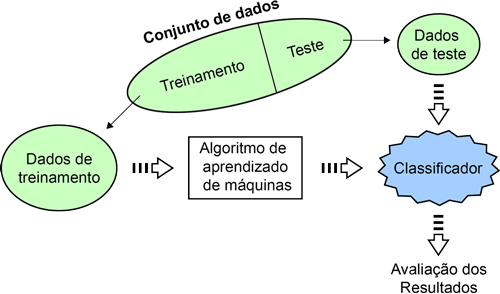
\includegraphics[scale=0.7]{figs/training-datasets-pequeno.png}
	\caption{\label{fig_1}Processo dos algoritmos de aprendizado de máquinas}
\end{figure}

Existe uma variedade de métodos para avaliar a performance de um classificador. É possível, por exemplo, selecionar uma porcentagem de um conjunto de dados para aplicar os algoritmos de aprendizado de máquinas e usar o resto para teste. O método de avaliação padrão e mais confiável é chamado \textit{cross-validation}. Neste caso, foi utilizado o \textit{10-fold cross-validation} que divide o conjunto em 10 partes iguais (as chamadas \textit{folds}), usa 9 partes dessa divisão para treinamento e guarda uma parte para teste, e depois, faz isso mais 9 vezes, sempre alternando a parte utilizada para teste, assim, uma determinada parte é usada 9 vezes para treinamento e uma para teste. O resultado é a média das 10 vezes que o algoritmo executou.

Os algoritmos de aprendizado de máquina que foram utilizados são o J48, um classificador em árvore, e o NaïveBayes, um classificador bayesiano.

J48 é uma variação de um famoso sistema chamado C4.5, descrito por Quinlan \cite{Quinlan1993} que usa árvores de decisão para construir um classificador (WEKA inclusive fornece uma visão da árvore gerada com todos os seus pesos).

NaïveBayes é um método probabilístico que possui duas assunções: que os atributos são igualmente importantes e estatisticamente independentes (essa assunção de independência nunca é 100\% correta, mas os métodos baseados nela geralmente funcionam bem na prática). Observando as métricas coletadas e o conjunto de dados gerado após a aplicação da pesquisa, esses dois métodos parecem servir bem aos propósitos deste estudo.

Foi utilizado também um terceiro algoritmo chamado \textit{AttributeSelectClassifier}, que na verdade usa um método de seleção de características (nesse caso, o \textit{GainRatio}) e um algoritmo para executar a classificação (nesse caso, J48 ou NaïveBayes). Esta é uma maneira mais apropriada para aplicar seleção de características porque assim o algoritmo seleciona as características no conjunto de treinamento, tornando os resultados mais confiáveis.

Por fim, para conduzir todas essas análises foi utilizado um modo do programa WEKA chamado EXPERIMENTER, que permite rodar o mesmo experimento mais de uma vez e determinar a média e o desvio padrão, para evitar falsos resultados otimistas ou pessimistas (alta ou baixa acurácia) devido à seleção de atributos nos conjuntos de treinamento e teste. Esse modo permite comparar os resultados de diferentes algoritmos.
























% ----------------------------------------------------------
% Referencial Teórico
% ----------------------------------------------------------
\chapter[Resultados Gerais]{Resultados Gerais (Todas Empresas)}

Seguindo os passos apresentados no capítulo anterior, serão mostrados os resultados da aplicação da pesquisa, a seleção de características executada no conjunto de dados gerados por essa pesquisa e a aplicação dos classificadores e suas respectivas acurácias na classificação dos desenvolvedores.

\section{Pesquisa}\label{secao4.2}
Primeiramente serão apresentados os dados coletados com a pesquisa. Onze respondentes (supervisores) forneceram 61 respostas (avaliações únicas de desenvolvedores). Em alguns casos, mais de um supervisor trabalham na mesma empresa, porém eles supervisionam diferente times. No total, oito empresas foram envolvidas na coleta de dados. Na tabela \ref{tabela2_1}, podemos ver, por empresa, quantos supervisores (que supervisionam diferentes times) responderam a pesquisa e quantos desenvolvedores foram avaliados.

Assim como mostrado na Seção \ref{caracterizacao_respondentes}, as empresas participantes são empresas que possuem uma área de desenvolvimento de software com ao menos um supervisor. Todas as empresas estão situadas na cidade de Uberlândia e trabalham em seus próprios produtos (não apenas desenvolvem software de maneira terceirizada), mas elas variam em tamanho, considerando quantidade de desenvolvedores como critério, setor de operação (ERP, Telecomunicações, etc), e podem variar em tecnologia utilizada.


\begin{table}[h]
	\caption{Relação dos participantes na pesquisa}
	\label{tabela2_1}
	\def\arraystretch{2}
	\begin{tabular}{|>{\centering\arraybackslash}p{3cm}|>{\centering\arraybackslash}p{5.75cm}|>{\centering\arraybackslash}p{5.75cm}|}
		\hline
		{\textbf{Empresa}} &
		\parbox{5.75cm}{\textbf{Quantidade de supervisores}} & 
		\parbox{5.75cm}{\textbf{Quantidade de desenvolvedores avaliados}} \\ \hline
		A                                      & 2                                                              & 20                                                                    \\ \hline
		B                                      & 1                                                              & 10                                                                    \\ \hline
		C                                      & 3                                                              & 20                                                                    \\ \hline
		D                                      & 1                                                              & 4                                                                     \\ \hline
		E                                      & 1                                                              & 3                                                                     \\ \hline
		F                                      & 1                                                              & 2                                                                     \\ \hline
		G                                      & 1                                                              & 1                                                                     \\ \hline
		H                                      & 1                                                              & 1                                                                     \\ \hline
		\textbf{total}                         & 11                                                             & 61                                                                    \\ \hline
	\end{tabular}
\end{table}

Foi pedido para os supervisores classificarem os desenvolvedores em 5 graus de importância. Esses graus de importância e a distribuição dos desenvolvedores avaliados neles é mostrado na \autoref{fig_3}.

\begin{figure}[h]
	\centering
	\includegraphics[scale=0.8]{figs/geral/imagem-classe-original.png}
	\caption{\label{fig_3}Distribuição dos desenvolvedores avaliados pelas classes de importância}
\end{figure}

Analisando os resultados da pesquisa, percebe-se que os supervisores podem ter sido, em certo nível, conservadores em classificar seus desenvolvedores nas classificações mais baixas de importância. Uma possível explicação para esse comportamento é o viés criado ao seguir a linha de raciocínio de que se o desenvolvedor possui baixa importância, ele não estaria na equipe.
Esse viés na classificação dos desenvolvedores impacta diretamente a acurácia dos classificadores, visto que eles usam a classe como base para tentar descobrir um padrão nos dados. Caso a classificação não tenha ficado clara para todos os respondentes, os algoritmos podem se confundir e apresentar erros leves, classificando um determinado indivíduo em classes similares, mas não à classe que ele realmente pertence. Esses erros em grande quantidade interferem e possuem um impacto negativo significativo na acurácia do classificador que é proposto neste estudo.

A partir dessa análise, juntamente com a análise da matriz de confusão gerada pela aplicação dos algoritmos descritos na Seção \ref{secao3.4}, decidiu-se agrupar os desenvolvedores em apenas duas classes, baseadas nas cinco classes originais de importância, como mostrado na \autoref{tabela3}, com o intuito de obter uma análise mais realística.

%inserir tabela 3

\begin{table}[h]
	\centering
	\caption{Novo conjunto de classes de desenvolvedores}
	\label{tabela3}
	\def\arraystretch{1.5}
	\begin{tabular}{|p{6cm}|p{8.5cm}|}
		\hline
		\textbf{Novo conjunto de classes}  & \textbf{Conjunto de classes originais} \\ \hline
		\multirow{2}{*}{Alta importância}  & Muito importante                       \\ \cline{2-2} 
		& Importante                             \\ \hline
		\multirow{3}{*}{Baixa importância} & Importância média                      \\ \cline{2-2} 
		& Pouco importante                       \\ \cline{2-2} 
		& Muito pouco importante                 \\ \hline
	\end{tabular}
\end{table}

Utilizando esse novo conjunto de classes para agrupar os desenvolvedores, obteve-se a distribuição mostrada na \autoref{fig_4}.

\begin{figure}[h]
	\centering
	\includegraphics[scale=0.8]{figs/geral/imagem-classe-alternativa.png}
	\caption{\label{fig_4}Distribuição dos desenvolvedores avaliados pela nova classe de importância}
\end{figure}

\section{Seleção de Características}\label{secao4.3}

Como explicado na Seção \ref{secao3.3}, foi utilizado o algoritmo \textit{GainRatio} para ordenar as características propostas, para prosseguir com a seleção de características. A \autoref{tabela4} mostra as características ordenadas pelo mérito médio (grau de influência da característica na classificação, calculado pelo algoritmo) resultante da aplicação do algoritmo usando as classes originais e a \autoref{tabela5} mostra a mesma visão, utilizando o novo conjunto de 2 classes. 

É possível notar algumas semelhanças e diferenças entre essas tabelas. as três primeiras características da primeira tabela, por exemplo, ocupam também as três primeiras posições na segunda, apesar de estarem em ordem diferente, o que mostra que a mudança do conjunto de classes não teve um impacto muito significativo na relevância dessas características. Porém, após as três primeiras, é possível notar algumas diferenças mais expressivas no posicionamento dos características, mostrando então um maior impacto nas características menos relevantes causada pela troca do conjunto de classes.

%inserir Tabela 4
\begin{table}[h]
	\caption{Ordenação das características (conjunto original de 5 classes)}
	\label{tabela4}
	\def\arraystretch{2}
	\begin{tabular}{|p{8.5cm}|>{\centering\arraybackslash}p{3cm}|>{\centering\arraybackslash}p{3cm}|}
		\hline
		\textbf{Características}                                                      & \textbf{Posição média} & \textbf{Mérito médio} \\ \hline
		Capacidade de resolução de problemas complexos                          & 1.4 +- 0.49                                 & 0.303 +- 0.03                                                                          \\ \hline
		Qual a sua avaliação sobre a produtividade do desenvolvedor em questão? & 1.6 +- 0.49                                 & 0.29  +- 0.022                                                                         \\ \hline
		Pró-atividade                                                           & 3.6 +- 0.92                                 & 0.226 +- 0.01                                                                          \\ \hline
		Experiência relevante                                                   & 4.8 +- 1.17                                 & 0.211 +- 0.014                                                                         \\ \hline
		Diversidade de habilidades                                              & 5.6 +- 1.36                                 & 0.202 +- 0.022                                                                         \\ \hline
		Conhecimento especializado                                              & 6.1 +- 2.51                                 & 0.2   +- 0.026                                                                         \\ \hline
		Tempo de trabalho (meses)                                               & 7.1 +- 1.37                                 & 0.184 +- 0.012                                                                         \\ \hline
		Criatividade                                                            & 7.4 +- 1.62                                 & 0.18  +- 0.021                                                                         \\ \hline
		Foco nos resultados                                                     & 8.7 +- 1.27                                 & 0.167 +- 0.017                                                                         \\ \hline
		Foco no cliente                                                         & 10 +- 2.45                                  & 0.148 +- 0.023                                                                         \\ \hline
		Principal comportamento do desenvolvedor                                & 11.1 +- 1.58                                & 0.14  +- 0.021                                                                         \\ \hline
		Comunicação com os colegas                                              & 11.6 +- 1.02                                & 0.137 +- 0.011                                                                         \\ \hline
		Organização e planejamento                                              & 12.3 +- 1.27                                & 0.122 +- 0.015                                                                         \\ \hline
		Liderança                                                               & 14.5 +- 1.2                                 & 0.097 +- 0.018                                                                         \\ \hline
		Empreendedorismo                                                        & 15 +- 0.89                                  & 0.087 +- 0.012                                                                         \\ \hline
		Disposição para ajudar colegas quando solicitado                        & 15.2 +- 0.6                                 & 0.084 +- 0.014                                                                         \\ \hline
	\end{tabular}
\end{table}
\clearpage
%inserir Tabela 5

\begin{table}[h]
	\caption{Ordenação das características (novo conjunto de 2 classes)}
	\label{tabela5}
	\def\arraystretch{2}
	\begin{tabular}{|p{8.5cm}|>{\centering\arraybackslash}p{3cm}|>{\centering\arraybackslash}p{3cm}|}
		\hline
		\textbf{Características}                                                      & \textbf{Posição média} & \textbf{Mérito médio} \\ \hline
		Pró-atividade                                                           & 1.2 +- 0.4             & 0.168 +- 0.01         \\ \hline
		Qual a sua avaliação sobre a produtividade do desenvolvedor em questão? & 1.9 +- 0.54            & 0.156 +- 0.017        \\ \hline
		Capacidade de resolução de problemas complexos                          & 3.2 +- 0.6             & 0.126 +- 0.013        \\ \hline
		Foco nos resultados                                                     & 4.8 +- 0.98            & 0.112 +- 0.018        \\ \hline
		Experiência relevante                                                   & 4.9 +- 1.3             & 0.107 +- 0.018        \\ \hline
		Criatividade                                                            & 6.5 +- 1.36            & 0.095 +- 0.008        \\ \hline
		Organização e planejamento                                              & 6.9 +- 2.21            & 0.09 +- 0.014         \\ \hline
		Diversidade de habilidades                                              & 8.1 +- 1.14            & 0.08 +- 0.011         \\ \hline
		Conhecimento especializado                                              & 9.2 +- 1.78            & 0.071 +- 0.013        \\ \hline
		Foco no cliente                                                         & 10.3 +- 1.95           & 0.063 +- 0.012        \\ \hline
		Tempo de trabalho (meses)                                               & 10.8 +- 1.08           & 0.063 +- 0.01         \\ \hline
		Disposição para ajudar colegas quando solicitado                        & 11.6 +- 2.24           & 0.057 +- 0.019        \\ \hline
		Liderança                                                               & 12 +- 0.89             & 0.052 +- 0.004        \\ \hline
		Comunicação com os colegas                                              & 13.6 +- 0.92           & 0.039 +- 0.009        \\ \hline
		Empreendedorismo                                                        & 15.5 +- 0.5            & 0.015 +- 0.005        \\ \hline
		Principal comportamento do desenvolvedor                                & 15.5 +- 0.5            & 0.016 +- 0.007        \\ \hline
	\end{tabular}
\end{table}
\clearpage

\section{Classificação}\label{secao4.4}

Considerando que as características foram ordenados, foi aplicado a técnica de seleção de características e usado apenas as características mais relevantes na classificação. Para determinar quantas características precisam ser selecionadas para se obter uma maior performance, foi conduzido um teste exaustivo (os classificadores rodaram com um crescente número de características selecionadas, de 2 a 16) e escolhido a configuração com melhor performance (8 características). A \autoref{tabela7.1} e a \autoref{tabela7.2} mostram então a aplicação exaustiva do algoritmo que associa a seleção de características com os algoritmos de classificação, para o J48 e para o NaïveBayes respectivamente.

A \autoref{tabela6} mostra os resultados da aplicação do algoritmo J48.Neste caso, o J48 não apresentou uma boa performance, com acurácia perto de 60\%, para o conjunto original de classes, porém já apresentou uma acurácia significativa ao ser aplicado sobre o novo conjunto de classes (80\% de acertos). No caso do J48, para ambos os conjuntos de classe, o classificador obteve a melhor performance utilizando apenas 2 características, como mostrado na \autoref{tabela7.1}.

NaïveBayes, como mostrado na \autoref{tabela7} obteve uma performance similar ao J48 quando aplicado no conjunto original de classes (acurácia perto de 61\%). Já para o novo conjunto de classes, NaïveBayes atingiu uma acurácia expressiva de 85\%. Ambos os melhores resultados do NaïveBayes foram atingidos utilizando 8 características, como mostra a \autoref{tabela7.2}.

%inserir Tabela 6

\begin{table}[h]
	\centering
	\caption{Aplicação do J48 para os diferentes conjuntos de classe }
	\label{tabela6}
	\def\arraystretch{1.5}
	\begin{tabular}{|p{7.25cm}|>{\centering\arraybackslash}p{7.25cm}|}
		\hline
		\textbf{Classe}                         & \textbf{Porcentagem de acertos} \\ \hline
		\textbf{Conjunto original de 5 classes} & 60.64\%                         \\ \hline
		\textbf{Conjunto com 2 classes}       & 80.14\%                         \\ \hline
	\end{tabular}
\end{table}

%inserir Tabela 7

\begin{table}[h]
	\centering
	\caption{Aplicação do NaïveBayes para os diferentes conjuntos de classe }
	\label{tabela7}
	\def\arraystretch{1.5}
	\begin{tabular}{|p{7.25cm}|>{\centering\arraybackslash}p{7.25cm}|}
		\hline
		\textbf{Classe}                         & \textbf{Porcentagem de acertos} \\ \hline
		\textbf{Conjunto original de 5 classes} & 61.12\%                         \\ \hline
		\textbf{Conjunto com 2 classes}       & 85.62\%                         \\ \hline
	\end{tabular}
\end{table}

\begin{table}[h]
	\centering
	\caption{Aplicação exaustiva do J48}
	\label{tabela7.1}
	\def\arraystretch{2}
	
	\begin{tabular}{|>{\centering\arraybackslash}p{3cm}|>{\centering\arraybackslash}p{5.75cm}|>{\centering\arraybackslash}p{5.75cm}|}
		\hline
		\parbox[l][1.5cm][c]{3cm}{\textbf{Número de \\características}} &
		\parbox[l][1.5cm][c]{5.75cm}{\textbf{\% de acertos - conjunto \\original de 5 classes}} &
		\parbox[l][1.5cm][c]{5.75cm}{\textbf{\% de acertos - conjunto \\de 2 classes}} \\ \hline
		2                                                                                                    & 60,64                                                                                                                                        & 80,14                                                                                                                               \\ \hline
		3                                                                                                    & 55,38                                                                                                                                        & 78,33                                                                                                                               \\ \hline
		4                                                                                                    & 58,55                                                                                                                                        & 77,67                                                                                                                               \\ \hline
		5                                                                                                    & 57,14                                                                                                                                        & 77,5                                                                                                                                \\ \hline
		6                                                                                                    & 56,31                                                                                                                                        & 77,02                                                                                                                               \\ \hline
		7                                                                                                    & 53,45                                                                                                                                        & 76,52                                                                                                                               \\ \hline
		8                                                                                                    & 51,88                                                                                                                                        & 75,88                                                                                                                               \\ \hline
		9                                                                                                    & 51,07                                                                                                                                        & 75,24                                                                                                                               \\ \hline
		10                                                                                                   & 50,6                                                                                                                                         & 74,74                                                                                                                               \\ \hline
		11                                                                                                   & 49,29                                                                                                                                        & 74,74                                                                                                                               \\ \hline
		12                                                                                                   & 48,64                                                                                                                                        & 74,74                                                                                                                               \\ \hline
		13                                                                                                   & 48,81                                                                                                                                        & 74,74                                                                                                                               \\ \hline
		14                                                                                                   & 48,14                                                                                                                                        & 74,74                                                                                                                               \\ \hline
		15                                                                                                   & 48,48                                                                                                                                        & 74,6                                                                                                                                \\ \hline
		16                                                                                                   & 48,48                                                                                                                                        & 74,6                                                                                                                                \\ \hline
	\end{tabular}
\end{table}

\begin{table}[h]
	\centering
	\caption{Aplicação exaustiva do NaïveBayes}
	\label{tabela7.2}
	\def\arraystretch{2}
	
	\begin{tabular}{|>{\centering\arraybackslash}p{3cm}|>{\centering\arraybackslash}p{5.75cm}|>{\centering\arraybackslash}p{5.75cm}|}
		\hline
		\parbox[l][1.5cm][c]{3cm}{\textbf{Número de \\características}} &
		\parbox[l][1.5cm][c]{5.75cm}{\textbf{\% de acertos - conjunto \\original de 5 classes}} &
		\parbox[l][1.5cm][c]{5.75cm}{\textbf{\% de acertos - conjunto \\de 2 classes}} \\ \hline
		2                                                                                                    & 60,02                                                                                                                                        & 80,81                                                                                                                               \\ \hline
		3                                                                                                    & 57,19                                                                                                                                        & 80,95                                                                                                                               \\ \hline
		4                                                                                                    & 55,79                                                                                                                                        & 82,38                                                                                                                               \\ \hline
		5                                                                                                    & 57,88                                                                                                                                        & 82,83                                                                                                                               \\ \hline
		6                                                                                                    & 59,52                                                                                                                                        & 85,62                                                                                                                               \\ \hline
		7                                                                                                    & 58,81                                                                                                                                        & 84,69                                                                                                                               \\ \hline
		8                                                                                                    & 61,12                                                                                                                                        & 85,21                                                                                                                               \\ \hline
		9                                                                                                    & 58,5                                                                                                                                         & 82,55                                                                                                                               \\ \hline
		10                                                                                                   & 58,52                                                                                                                                        & 82,55                                                                                                                               \\ \hline
		11                                                                                                   & 59,21                                                                                                                                        & 82,21                                                                                                                               \\ \hline
		12                                                                                                   & 58,71                                                                                                                                        & 82,55                                                                                                                               \\ \hline
		13                                                                                                   & 59,02                                                                                                                                        & 83,55                                                                                                                               \\ \hline
		14                                                                                                   & 59,48                                                                                                                                        & 83,88                                                                                                                               \\ \hline
		15                                                                                                   & 58,69                                                                                                                                        & 84,17                                                                                                                               \\ \hline
		16                                                                                                   & 58,57                                                                                                                                        & 83,52                                                                                                                               \\ \hline
	\end{tabular}
\end{table}




% ----------------------------------------------------------
% Referencial Teórico
% ----------------------------------------------------------
\chapter[Resultados Individuais por Empresa]{Resultados Individuais por Empresa}

Em nossa pesquisa, para as 8 empresas que participaram, 3 delas atingiram o número mínimo de respostas que permitem uma análise individual da empresa (10 avaliações de desenvolvedores). Nós iremos mostrar nesse capítulo o resultado que obtivemos analisando essas 3 empresas. Para proteger as informações dessas empresas, elas não serão identificadas. Nos referenciaremos à elas então como “Empresa A”, “Empresa B” e “Empresa C”.

\section{Análise das Empresas}

Para cada uma das 3 empresas, faremos a análise utilizando os dois conjuntos de classes, apontando as diferenças nos resultados. Mostraremos então a distribuição dos desenvolvedores ao longo dos dois conjuntos de classes, a seleção de características executadas no conjunto de dados resultantes da pesquisa respondida pelos supervisores das respectivas empresas e o resultado da aplicação dos algoritmos de classificação (dados de diferentes times, porém pertencentes à mesma empresa foram mesclados para obtermos uma visão geral da empresa).

Assim como fizemos com o conjunto de dados que representava todas as empresas, aplicamos aqui os algoritmos de classificação J48 e NaïveBayes nos dados fornecidos pelas respectivas empresas, utilizando tanto o conjunto original de 5 classes quanto o conjunto de 2 classes. 

Como explicado na Seção \ref{secao3.4}, para associar a seleção de características com os algoritmos de classificação da maneira correta, utilizaremos o Algoritmo AttributeSelectedClassifier, usando o algoritmo GainRatioAttributeEval para selecionar os atributos mais relevantes. E da mesma maneira que foi realizado a seleção de características ao analisarmos o conjunto de dados de todas as empresas (apresentado na Seção \ref{secao4.4}), a quantidade de características ideal que maximiza a acurácia dos classificadores é escolhida através de um teste exaustivo, começando com apenas duas características e aumentando uma a uma até chegar nas dezesseis características apresentadas na \autoref{tabela2} (já começamos com um número maior que 1 pois o objetivo não é encontrar correlação de alguma característica em específico com a classe, e sim encontrar um padrão na combinação de características que se correlacione com a importância dada pelo supervisor).

\subsection{Análise da Empresa A}

\subsubsection{Pesquisa}

A empresa A obteve avaliações de 2 supervisores. Como eram times com propósitos bem diferentes, consideramos apenas as avaliações de um dos times para representar a Empresa A, visto que o segundo não obteve avaliações suficientes para ser analisado individualmente. Logo, o time avaliado obteve 19 avaliações de desenvolvedores. A \autopageref{fig_7} e a \autoref{fig_8} mostram a distribuição dos desenvolvedores pelo conjunto de classes original e pelo conjunto de 2 classes, respectivamente.


\begin{figure}[h]
	\centering
	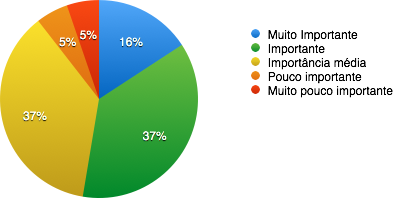
\includegraphics[scale=0.8]{figs/empresa_a/imagem-classe-original.png}
	\caption{\label{fig_7}Distribuição dos desenvolvedores pelo conjunto original de 5 classes (Empresa A)}
\end{figure}

\begin{figure}[h]
	\centering
	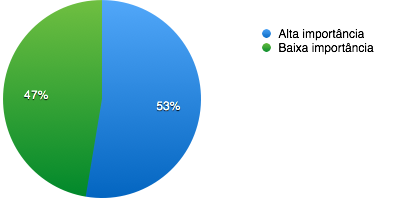
\includegraphics[scale=0.8]{figs/empresa_a/imagem-classe-alternativa.png}
	\caption{\label{fig_8}Distribuição dos desenvolvedores pelo conjunto de 2 classes (Empresa A)}
\end{figure}

\subsubsection{Seleção de Características}
O resultado da aplicação do algoritmo de seleção de características para o conjunto original de 5 classes e para o conjunto de 2 classes é apresentado na \autoref{tabela8} e na \autoref{tabela9} respectivamente.

%inserir Tabela 8
\begin{table}[h]
	\caption{Ordenação dos atributos da Empresa A (conjunto original de 5 classes)}
	\label{tabela8}
	\def\arraystretch{2}
	\begin{tabular}{|p{8.5cm}|>{\centering\arraybackslash}p{3cm}|>{\centering\arraybackslash}p{3cm}|}
		\hline
		\textbf{Atributos}                                                      & \textbf{Posição média} & \textbf{Mérito médio} \\ \hline
		Capacidade de resolução de problemas complexos                          & 1.5 +- 0.81            & 0.582 +- 0.038        \\ \hline
		Foco nos resultados                                                     & 2.6 +- 1.02            & 0.519 +- 0.047        \\ \hline
		Criatividade                                                            & 3 +- 1                 & 0.504 +- 0.035        \\ \hline
		Pró-atividade                                                           & 5.1 +- 2.12            & 0.456 +- 0.048        \\ \hline
		Foco no cliente                                                         & 6.4 +- 1.96            & 0.437 +- 0.04         \\ \hline
		Diversidade de habilidades                                              & 6.5 +- 1.91            & 0.435 +- 0.025        \\ \hline
		Experiência relevante                                                   & 6.9 +- 2.39            & 0.427 +- 0.035        \\ \hline
		Conhecimento especializado                                              & 8.9 +- 3.05            & 0.396 +- 0.053        \\ \hline
		Principal comportamento do desenvolvedor                                & 9.4 +- 2.91            & 0.384 +- 0.058        \\ \hline
		Qual a sua avaliação sobre a produtividade do desenvolvedor em questão? & 9.8 +- 2.44            & 0.383 +- 0.041        \\ \hline
		Comunicação com os colegas                                              & 10.5 +- 2.16           & 0.371 +- 0.051        \\ \hline
		Empreendedorismo                                                        & 11.7 +- 1.79           & 0.351 +- 0.047        \\ \hline
		Disposição para ajudar colegas quando solicitado                        & 12.1 +- 2.62           & 0.348 +- 0.05         \\ \hline
		Organização e planejamento                                              & 12.6 +- 2.24           & 0.336 +- 0.042        \\ \hline
		Tempo de trabalho (meses)                                               & 14.5 +- 4.5            & 0.064 +- 0.192        \\ \hline
		Liderança                                                               & 14.5 +- 0.81           & 0.285 +- 0.063        \\ \hline
	\end{tabular}
\end{table}
\clearpage

%inserir Tabela 9
\begin{table}[h]
	\caption{Ordenação dos atributos da Empresa A (conjunto de 2 classes)}
	\label{tabela9}
	\def\arraystretch{2}
	\begin{tabular}{|p{8.5cm}|>{\centering\arraybackslash}p{3cm}|>{\centering\arraybackslash}p{3cm}|}
		\hline
		\textbf{Atributos}                                                      & \textbf{Posição média} & \textbf{Mérito médio} \\ \hline
		Pró-atividade                                                           & 1.2 +- 0.4             & 0.323 +- 0.021        \\ \hline
		Capacidade de resolução de problemas complexos                          & 2.4 +- 0.8             & 0.298 +- 0.032        \\ \hline
		Comunicação com os colegas                                              & 4 +- 1.48              & 0.254 +- 0.024        \\ \hline
		Foco nos resultados                                                     & 5 +- 1.48              & 0.23 +- 0.029         \\ \hline
		Criatividade                                                            & 6.7 +- 1.68            & 0.206 +- 0.025        \\ \hline
		Qual a sua avaliação sobre a produtividade do desenvolvedor em questão? & 7.5 +- 2.01            & 0.187 +- 0.026        \\ \hline
		Organização e planejamento                                              & 7.8 +- 3.22            & 0.191 +- 0.035        \\ \hline
		Conhecimento especializado                                              & 8.2 +- 3.28            & 0.189 +- 0.056        \\ \hline
		Experiência relevante                                                   & 9.2 +- 3.12            & 0.173 +- 0.04         \\ \hline
		Empreendedorismo                                                        & 10.2 +- 3.22           & 0.171 +- 0.037        \\ \hline
		Principal comportamento do desenvolvedor                                & 10.4 +- 3.8            & 0.172 +- 0.052        \\ \hline
		Disposição para ajudar colegas quando solicitado                        & 11.1 +- 4.35           & 0.156 +- 0.049        \\ \hline
		Foco no cliente                                                         & 11.2 +- 1.72           & 0.158 +- 0.02         \\ \hline
		Liderança                                                               & 13 +- 2.53             & 0.137 +- 0.039        \\ \hline
		Diversidade de habilidades                                              & 13.4 +- 3.1            & 0.136 +- 0.046        \\ \hline
		Tempo de trabalho (meses)                                               & 14.7 +- 1.68           & 0.123 +- 0.022        \\ \hline
	\end{tabular}
\end{table}
\clearpage
\subsubsection{Classificação}

A \autoref{tabela10} e a \autoref{tabela11} apresentam os melhores resultados obtidos através da aplicação dos algoritmos J48 e NaïveBayes nos dados da Empresa A, respectivamente. Os algoritmos foram aplicados em ambos conjunto original de 5 classes e no conjunto de 2 classes. 

A \autoref{tabela11_1} e a \autoref{tabela11_2} mostram a aplicação exaustiva do algoritmo que associa a seleção de características com os algoritmos de classificação, para o J48 e para o NaïveBayes respectivamente.

Observando o teste exaustivo do J48, pudemos notar que ele obteve uma melhor performance utilizando um pequeno número de características ao realizar a classificação. No caso do conjunto original de 5 classes, os melhores resultados foram obtidos selecionando de 2 a 4 características, e ao ser aplicado utilizando o conjunto de 2 classes, a melhor acurácia foi obtida selecionando apenas 2 características. É importante ressaltar também o aumento de aproximadamente 20\% na acurácia do classificador utilizando a segunda classe de dados.

Diferentemente do J48, o NaïveBayes obteve uma melhor performance ao selecionar um maior número de características, de 13 a 15 no conjunto original de 5 classes e acima de 7 no conjunto de 2 classes. O NaïveBayes também teve uma melhoria de performance considerável ao utilizar o novo conjunto de dados (11\%).

%inserir Tabela 10
\begin{table}[h]
	\caption{Aplicação do J48 para os diferentes conjuntos de classe da Empresa A}
	\label{tabela10}
	\def\arraystretch{1.5}
	\begin{tabular}{|p{7.25cm}|>{\centering\arraybackslash}p{7.25cm}|}
		\hline
		\textbf{Classe}                         & \textbf{Porcentagem de acertos} \\ \hline
		\textbf{Conjunto original de 5 classes} & 59\%                         \\ \hline
		\textbf{Conjunto com 2 classes}       & 79.50\%                         \\ \hline
	\end{tabular}
\end{table}

%inserir Tabela 11
\begin{table}[h]
	\caption{Aplicação do NaïveBayes para os diferentes conjuntos de classe da Empresa A}
	\label{tabela11}
	\def\arraystretch{1.5}
	\begin{tabular}{|p{7.25cm}|>{\centering\arraybackslash}p{7.25cm}|}
		\hline
		\textbf{Classe}                         & \textbf{Porcentagem de acertos} \\ \hline
		\textbf{Conjunto original de 5 classes} & 68.50\%                         \\ \hline
		\textbf{Conjunto com 2 classes}       & 79.50\%                         \\ \hline
	\end{tabular}
\end{table}

\begin{table}[h]
	\centering
	\caption{Aplicação exaustiva do J48 para a empresa A}
	\label{tabela11_1}
	\def\arraystretch{2}
	
	\begin{tabular}{|>{\centering\arraybackslash}p{3cm}|>{\centering\arraybackslash}p{5.75cm}|>{\centering\arraybackslash}p{5.75cm}|}
		\hline
		\parbox[l][1.5cm][c]{3cm}{\textbf{Número de \\características}} &
		\parbox[l][1.5cm][c]{5.75cm}{\textbf{\% de acertos - conjunto \\original de 5 classes}} &
		\parbox[l][1.5cm][c]{5.75cm}{\textbf{\% de acertos - conjunto \\de 2 classes}} \\ \hline

		2                                                                                                    & 57                                                                                                                                           & 79,5                                                                                                                                \\ \hline
		3                                                                                                    & 59                                                                                                                                           & 76                                                                                                                                  \\ \hline
		4                                                                                                    & 59                                                                                                                                           & 75,5                                                                                                                                \\ \hline
		5                                                                                                    & 59                                                                                                                                           & 75,5                                                                                                                                \\ \hline
		6                                                                                                    & 57                                                                                                                                           & 75,5                                                                                                                                \\ \hline
		7                                                                                                    & 57                                                                                                                                           & 75,5                                                                                                                                \\ \hline
		8                                                                                                    & 57                                                                                                                                           & 75,5                                                                                                                                \\ \hline
		9                                                                                                    & 57                                                                                                                                           & 75,5                                                                                                                                \\ \hline
		10                                                                                                   & 56,5                                                                                                                                         & 75,5                                                                                                                                \\ \hline
		11                                                                                                   & 56,5                                                                                                                                         & 74,5                                                                                                                                \\ \hline
		12                                                                                                   & 56,5                                                                                                                                         & 74,5                                                                                                                                \\ \hline
		13                                                                                                   & 56,5                                                                                                                                         & 74,5                                                                                                                                \\ \hline
		14                                                                                                   & 56,5                                                                                                                                         & 74,5                                                                                                                                \\ \hline
		15                                                                                                   & 56,5                                                                                                                                         & 74,5                                                                                                                                \\ \hline
		16                                                                                                   & 56,5                                                                                                                                         & 74,5                                                                                                                                \\ \hline
	\end{tabular}
\end{table}
\clearpage

\begin{table}[h]
	\centering
	\caption{Aplicação exaustiva do NaïveBayes para a empresa A}
	\label{tabela11_2}
	\def\arraystretch{2}
	
	\begin{tabular}{|>{\centering\arraybackslash}p{3cm}|>{\centering\arraybackslash}p{5.75cm}|>{\centering\arraybackslash}p{5.75cm}|}
		\hline
		\parbox[l][1.5cm][c]{3cm}{\textbf{Número de \\características}} &
		\parbox[l][1.5cm][c]{5.75cm}{\textbf{\% de acertos - conjunto \\original de 5 classes}} &
		\parbox[l][1.5cm][c]{5.75cm}{\textbf{\% de acertos - conjunto \\de 2 classes}} \\ \hline

		2                                                                                                    & 58                                                                                                                                           & 78                                                                                                                                  \\ \hline
		3                                                                                                    & 59,5                                                                                                                                         & 73                                                                                                                                  \\ \hline
		4                                                                                                    & 55,5                                                                                                                                         & 68                                                                                                                                  \\ \hline
		5                                                                                                    & 58                                                                                                                                           & 71,5                                                                                                                                \\ \hline
		6                                                                                                    & 57                                                                                                                                           & 75,5                                                                                                                                \\ \hline
		7                                                                                                    & 58                                                                                                                                           & 78                                                                                                                                  \\ \hline
		8                                                                                                    & 59                                                                                                                                           & 79,5                                                                                                                                \\ \hline
		9                                                                                                    & 58                                                                                                                                           & 79,5                                                                                                                                \\ \hline
		10                                                                                                   & 64                                                                                                                                           & 79,5                                                                                                                                \\ \hline
		11                                                                                                   & 62,5                                                                                                                                         & 79,5                                                                                                                                \\ \hline
		12                                                                                                   & 67                                                                                                                                           & 79,5                                                                                                                                \\ \hline
		13                                                                                                   & 68,5                                                                                                                                         & 79,5                                                                                                                                \\ \hline
		14                                                                                                   & 68,5                                                                                                                                         & 79,5                                                                                                                                \\ \hline
		15                                                                                                   & 68,5                                                                                                                                         & 79,5                                                                                                                                \\ \hline
		16                                                                                                   & 55,5                                                                                                                                         & 79,5                                                                                                                                \\ \hline
	\end{tabular}
\end{table}
\clearpage

\subsection{Análise da Empresa B}

\subsubsection{Pesquisa}

A Empresa B obteve 10 avaliações de desenvolvedores feitas por um único supervisor. A \autoref{fig_11} e a \autoref{fig_12} mostram a distribuição dos desenvolvedores pelo conjunto de classes original e pelo conjunto de 2 classes, respectivamente.

\begin{figure}[h]
	\centering
	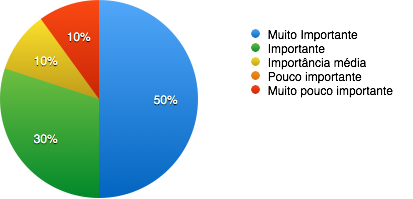
\includegraphics[scale=0.8]{figs/empresa_b/imagem-classe-original.png}
	\caption{\label{fig_11}Distribuição dos desenvolvedores pelo conjunto original de 5 classes (Empresa B)}
\end{figure}

\begin{figure}[h]
	\centering
	\includegraphics[scale=0.8]{figs/empresa_b/imagem-classe-alternativa.png}
	\caption{\label{fig_12}Distribuição dos desenvolvedores pelo conjunto de 2 classes (Empresa B)}
\end{figure}

\subsubsection{Seleção de Características}
O resultado da aplicação do algoritmo de seleção de características para o conjunto original de 5 classes e para o conjunto de 2 classes é apresentado na \autoref{tabela12} e na \autoref{tabela13} respectivamente.

%inserir Tabela 12
\begin{table}[h]
	\caption{Ordenação dos atributos da Empresa B (conjunto original de 5 classes)}
	\label{tabela12}
	\def\arraystretch{2}
	\begin{tabular}{|p{8.5cm}|>{\centering\arraybackslash}p{3cm}|>{\centering\arraybackslash}p{3cm}|}
		\hline
		\textbf{Atributos}                                                      & \textbf{Posição média} & \textbf{Mérito médio} \\ \hline
		Capacidade de resolução de problemas complexos                          & 1.3 +- 0.46            & 0.772 +- 0.078        \\ \hline
		Liderança                                                               & 2.4 +- 1.02            & 0.652 +- 0.118        \\ \hline
		Tempo de trabalho (meses)                                               & 4.6 +- 1.43            & 0.562 +- 0.063        \\ \hline
		Foco nos resultados                                                     & 5 +- 3.63              & 0.611 +- 0.179        \\ \hline
		Experiência relevante                                                   & 5.3 +- 3.29            & 0.611 +- 0.179        \\ \hline
		Organização e planejamento                                              & 6.4 +- 1.8             & 0.506 +- 0.073        \\ \hline
		Conhecimento especializado                                              & 6.7 +- 2.1             & 0.515 +- 0.094        \\ \hline
		Diversidade de habilidades                                              & 8 +- 1.48              & 0.456 +- 0.06         \\ \hline
		Criatividade                                                            & 9.7 +- 2.79            & 0.413 +- 0.119        \\ \hline
		Qual a sua avaliação sobre a produtividade do desenvolvedor em questão? & 11.1 +- 2.43           & 0.361 +- 0.076        \\ \hline
		Pró-atividade                                                           & 11.2 +- 1.54           & 0.35 +- 0.04          \\ \hline
		Foco no cliente                                                         & 11.2 +- 4.04           & 0.373 +- 0.133        \\ \hline
		Empreendedorismo                                                        & 11.4 +- 1.74           & 0.36 +- 0.079         \\ \hline
		Disposição para ajudar colegas quando solicitado                        & 12.4 +- 1.85           & 0.339 +- 0.08         \\ \hline
		Comunicação com os colegas                                              & 13.6 +- 2.15           & 0.318 +- 0.087        \\ \hline
		Principal comportamento do desenvolvedor                                & 15.7 +- 0.64           & 0.235 +- 0.048        \\ \hline
	\end{tabular}
\end{table}
\clearpage

%inserir Tabela 13
\begin{table}[h]
	\caption{Ordenação dos atributos da Empresa B (conjunto de 2 classes)}
	\label{tabela13}
	\def\arraystretch{2}
	\begin{tabular}{|p{8.5cm}|>{\centering\arraybackslash}p{3cm}|>{\centering\arraybackslash}p{3cm}|}
		\hline
		\textbf{Atributos}                                                      & \textbf{Posição média} & \textbf{Mérito médio} \\ \hline
		Foco nos resultados                                                     & 2.9 +- 4.41            & 0.327 +- 0.131        \\ \hline
		Comunicação com os colegas                                              & 3.3 +- 1.42            & 0.244 +- 0.067        \\ \hline
		Experiência relevante                                                   & 3.4 +- 4.25            & 0.327 +- 0.131        \\ \hline
		Criatividade                                                            & 4.1 +- 2.07            & 0.26 +- 0.069         \\ \hline
		Capacidade de resolução de problemas complexos                          & 5.6 +- 1.56            & 0.151 +- 0.052        \\ \hline
		Pró-atividade                                                           & 8.1 +- 3.14            & 0.112 +- 0.028        \\ \hline
		Principal comportamento do desenvolvedor                                & 8.1 +- 3.18            & 0.112 +- 0.028        \\ \hline
		Tempo de trabalho (meses)                                               & 8.6 +- 2.29            & 0.109 +- 0.033        \\ \hline
		Diversidade de habilidades                                              & 8.6 +- 3.5             & 0.119 +- 0.06         \\ \hline
		Qual a sua avaliação sobre a produtividade do desenvolvedor em questão? & 9.4 +- 1.74            & 0.093 +- 0.022        \\ \hline
		Empreendedorismo                                                        & 9.6 +- 1.85            & 0.093 +- 0.022        \\ \hline
		Disposição para ajudar colegas quando solicitado                        & 11.3 +- 1.42           & 0.063 +- 0.02         \\ \hline
		Conhecimento especializado                                              & 12.7 +- 1.42           & 0.043 +- 0.026        \\ \hline
		Organização e planejamento                                              & 12.9 +- 2.84           & 0.031 +- 0.043        \\ \hline
		Foco no cliente                                                         & 13.3 +- 3.23           & 0.031 +- 0.043        \\ \hline
		Liderança                                                               & 14.1 +- 3.67           & 0.023 +- 0.04         \\ \hline
	\end{tabular}
\end{table}
\clearpage

\subsubsection{Classificação}

A \autoref{tabela14} e a \autoref{tabela15} apresentam os melhores resultados obtidos através da aplicação dos algoritmos J48 e NaïveBayes nos dados da empresa B, respectivamente. Os algoritmos foram aplicados em ambos conjunto original de 5 classes e no conjunto de 2 classes.

A \autoref{tabela15_1} e a \autoref{tabela15_2} mostram a aplicação exaustiva do algoritmo que associa a seleção de características com os algoritmos de classificação, para o J48 e para o NaïveBayes respectivamente.

Observando o teste exaustivo do J48, pudemos notar que, para o conjunto de classes original, o algoritmo obteve uma melhor performance utilizando um menor número de características (de 2 a 6). Já ao utilizar o conjunto de 2 classes, o classificador obteve a mesma acurácia independentemente do número de características utilizado. Utilizando o segundo conjunto de classes, o J48 teve um aumento de 10\% em sua acurácia final.

No caso da Empresa B, o algoritmo NaïveBayes obteve uma performance extremamente semelhante ao J48, mantendo a performance praticamente constante de acordo com a variação das características selecionadas, obtendo uma melhoria de 10\% ao utilizar o conjunto de 2 classes, e obtendo uma acurácia final de 80\%. 

%inserir Tabela 14
\begin{table}[h]
	\caption{Aplicação do J48 para os diferentes conjuntos de classe da Empresa B}
	\label{tabela14}
	\def\arraystretch{1.5}
	\begin{tabular}{|p{7.25cm}|>{\centering\arraybackslash}p{7.25cm}|}
		\hline
		\textbf{Classe}                         & \textbf{Porcentagem de acertos} \\ \hline
		\textbf{Conjunto original de 5 classes} & 70\%                         \\ \hline
		\textbf{Conjunto com 2 classes}       & 80\%                         \\ \hline
	\end{tabular}
\end{table}

%inserir Tabela 15
\begin{table}[h]
	\caption{Aplicação do NaïveBayes para os diferentes conjuntos de classe da Empresa B}
	\label{tabela15}
	\def\arraystretch{1.5}
	\begin{tabular}{|p{7.25cm}|>{\centering\arraybackslash}p{7.25cm}|}
		\hline
		\textbf{Classe}                         & \textbf{Porcentagem de acertos} \\ \hline
		\textbf{Conjunto original de 5 classes} & 70\%                         \\ \hline
		\textbf{Conjunto com 2 classes}       & 80\%                         \\ \hline
	\end{tabular}
\end{table}

\begin{table}[h]
	\centering
	\caption{Aplicação exaustiva do J48 para a empresa B}
	\label{tabela15_1}
	\def\arraystretch{2}
	
	\begin{tabular}{|>{\centering\arraybackslash}p{3cm}|>{\centering\arraybackslash}p{5.75cm}|>{\centering\arraybackslash}p{5.75cm}|}
		\hline
		\parbox[l][1.5cm][c]{3cm}{\textbf{Número de \\características}} &
		\parbox[l][1.5cm][c]{5.75cm}{\textbf{\% de acertos - conjunto \\original de 5 classes}} &
		\parbox[l][1.5cm][c]{5.75cm}{\textbf{\% de acertos - conjunto \\de 2 classes}} \\ \hline

		2                                                                                                    & 70                                                                                                                                           & 80                                                                                                                                  \\ \hline
		3                                                                                                    & 70                                                                                                                                           & 80                                                                                                                                  \\ \hline
		4                                                                                                    & 70                                                                                                                                           & 80                                                                                                                                  \\ \hline
		5                                                                                                    & 70                                                                                                                                           & 80                                                                                                                                  \\ \hline
		6                                                                                                    & 70                                                                                                                                           & 80                                                                                                                                  \\ \hline
		7                                                                                                    & 70                                                                                                                                           & 80                                                                                                                                  \\ \hline
		8                                                                                                    & 60                                                                                                                                           & 80                                                                                                                                  \\ \hline
		9                                                                                                    & 60                                                                                                                                           & 80                                                                                                                                  \\ \hline
		10                                                                                                   & 60                                                                                                                                           & 80                                                                                                                                  \\ \hline
		11                                                                                                   & 60                                                                                                                                           & 80                                                                                                                                  \\ \hline
		12                                                                                                   & 60                                                                                                                                           & 80                                                                                                                                  \\ \hline
		13                                                                                                   & 60                                                                                                                                           & 80                                                                                                                                  \\ \hline
		14                                                                                                   & 60                                                                                                                                           & 80                                                                                                                                  \\ \hline
		15                                                                                                   & 60                                                                                                                                           & 80                                                                                                                                  \\ \hline
		16                                                                                                   & 60                                                                                                                                           & 80                                                                                                                                  \\ \hline
	\end{tabular}
\end{table}
\clearpage

\begin{table}[h]
	\centering
	\caption{Aplicação exaustiva do NaïveBayes para a empresa B}
	\label{tabela15_2}
	\def\arraystretch{2}
	
	\begin{tabular}{|>{\centering\arraybackslash}p{3cm}|>{\centering\arraybackslash}p{5.75cm}|>{\centering\arraybackslash}p{5.75cm}|}
		\hline
		\parbox[l][1.5cm][c]{3cm}{\textbf{Número de \\características}} &
		\parbox[l][1.5cm][c]{5.75cm}{\textbf{\% de acertos - conjunto \\original de 5 classes}} &
		\parbox[l][1.5cm][c]{5.75cm}{\textbf{\% de acertos - conjunto \\de 2 classes}} \\ \hline

		2                                                                                                    & 70                                                                                                                                           & 70                                                                                                                                  \\ \hline
		3                                                                                                    & 70                                                                                                                                           & 80                                                                                                                                  \\ \hline
		4                                                                                                    & 70                                                                                                                                           & 80                                                                                                                                  \\ \hline
		5                                                                                                    & 70                                                                                                                                           & 80                                                                                                                                  \\ \hline
		6                                                                                                    & 70                                                                                                                                           & 80                                                                                                                                  \\ \hline
		7                                                                                                    & 70                                                                                                                                           & 70                                                                                                                                  \\ \hline
		8                                                                                                    & 70                                                                                                                                           & 80                                                                                                                                  \\ \hline
		9                                                                                                    & 70                                                                                                                                           & 80                                                                                                                                  \\ \hline
		10                                                                                                   & 70                                                                                                                                           & 80                                                                                                                                  \\ \hline
		11                                                                                                   & 70                                                                                                                                           & 80                                                                                                                                  \\ \hline
		12                                                                                                   & 70                                                                                                                                           & 80                                                                                                                                  \\ \hline
		13                                                                                                   & 70                                                                                                                                           & 80                                                                                                                                  \\ \hline
		14                                                                                                   & 70                                                                                                                                           & 80                                                                                                                                  \\ \hline
		15                                                                                                   & 70                                                                                                                                           & 80                                                                                                                                  \\ \hline
		16                                                                                                   & 70                                                                                                                                           & 80                                                                                                                                  \\ \hline
	\end{tabular}
\end{table}
\clearpage

\subsection{Análise da Empresa C}

\subsubsection{Pesquisa}

A Empresa C obteve 18 avaliaçãos de desenvolvedores, dadas por 2 diferentes supervisores. Apesar de serem times diferentes, ambos fazem parte da mesma indústria de software, por isso resolvemos mesclar os dados e fazer uma avaliação conjunta. A Empresa C também obteve mais 2 avaliações dadas por um terceiro supervisor, mas os dados foram excluídos dessa análise pelo propósito desse time ser bastante diferente dos dois primeiros. A \autoref{fig_15} e a \autoref{fig_16} mostram a distribuição dos desenvolvedores pelo conjunto de classes original e pelo conjunto de 2 classes, respectivamente. 

\begin{figure}[h]
	\centering
	\includegraphics[scale=0.8]{figs/empresa_c/imagem-classe-original.png}
	\caption{\label{fig_15}Distribuição dos desenvolvedores pelo conjunto original de 5 classes (Empresa C)}
\end{figure}

\begin{figure}[h]
	\centering
	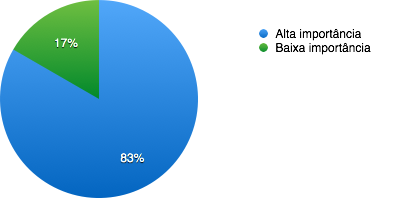
\includegraphics[scale=0.8]{figs/empresa_c/imagem-classe-alternativa.png}
	\caption{\label{fig_16}Distribuição dos desenvolvedores pelo conjunto de 2 classes (Empresa C)}
\end{figure}

\subsubsection{Seleção de Características}
O resultado da aplicação do algoritmo de seleção de características para o conjunto original de 5 classes e para o conjunto de 2 classes é apresentado na \autoref{tabela16} e na \autoref{tabela17} respectivamente.

%inserir Tabela 16
\begin{table}[h]
	\caption{Ordenação dos atributos da Empresa C (conjunto original de 5 classes)}
	\label{tabela16}
	\def\arraystretch{2}
	\begin{tabular}{|p{8.5cm}|>{\centering\arraybackslash}p{3cm}|>{\centering\arraybackslash}p{3cm}|}
		\hline
		\textbf{Atributos}                                                      & \textbf{Posição média} & \textbf{Mérito médio} \\ \hline
		Capacidade de resolução de problemas complexos                          & 1.1 +- 0.3             & 0.643 +- 0.044        \\ \hline
		Experiência relevante                                                   & 2.2 +- 0.4             & 0.581 +- 0.037        \\ \hline
		Conhecimento especializado                                              & 3.3 +- 0.9             & 0.518 +- 0.058        \\ \hline
		Qual a sua avaliação sobre a produtividade do desenvolvedor em questão? & 3.4 +- 0.66            & 0.504 +- 0.036        \\ \hline
		Diversidade de habilidades                                              & 5.2 +- 0.6             & 0.386 +- 0.046        \\ \hline
		Principal comportamento do desenvolvedor                                & 6.4 +- 0.8             & 0.338 +- 0.048        \\ \hline
		Comunicação com os colegas                                              & 8.1 +- 1.45            & 0.301 +- 0.029        \\ \hline
		Foco nos resultados                                                     & 8.5 +- 2.77            & 0.3 +- 0.08           \\ \hline
		Empreendedorismo                                                        & 9.6 +- 2.06            & 0.275 +- 0.037        \\ \hline
		Pró-atividade                                                           & 10.7 +- 2              & 0.267 +- 0.058        \\ \hline
		Tempo de trabalho (meses)                                               & 11.2 +- 1.66           & 0.261 +- 0.035        \\ \hline
		Foco no cliente                                                         & 11.3 +- 1.68           & 0.255 +- 0.045        \\ \hline
		Criatividade                                                            & 11.9 +- 2.55           & 0.246 +- 0.056        \\ \hline
		Liderança                                                               & 13.6 +- 2.01           & 0.21 +- 0.055         \\ \hline
		Organização e planejamento                                              & 14.2 +- 1.54           & 0.196 +- 0.042        \\ \hline
		Disposição para ajudar colegas quando solicitado                        & 15.3 +- 0.78           & 0.186 +- 0.044        \\ \hline
	\end{tabular}
\end{table}
\clearpage

%inserir Tabela 17
\begin{table}[h]
	\caption{Ordenação dos atributos da Empresa C (conjunto de 2 classes)}
	\label{tabela17}
	\def\arraystretch{2}
	\begin{tabular}{|p{8.5cm}|>{\centering\arraybackslash}p{3cm}|>{\centering\arraybackslash}p{3cm}|}
		\hline
		\textbf{Atributos}                                                      & \textbf{Posição média} & \textbf{Mérito médio} \\ \hline
		Conhecimento especializado                                              & 1 +- 0                 & 0.26 +- 0.028         \\ \hline
		Experiência relevante                                                   & 2.3 +- 0.46            & 0.24 +- 0.026         \\ \hline
		Qual a sua avaliação sobre a produtividade do desenvolvedor em questão? & 3.1 +- 0.83            & 0.227 +- 0.035        \\ \hline
		Capacidade de resolução de problemas complexos                          & 4 +- 0.45              & 0.216 +- 0.029        \\ \hline
		Diversidade de habilidades                                              & 5.6 +- 0.66            & 0.179 +- 0.027        \\ \hline
		Disposição para ajudar colegas quando solicitado                        & 6 +- 1.55              & 0.172 +- 0.034        \\ \hline
		Foco nos resultados                                                     & 7.1 +- 1.51            & 0.16 +- 0.03          \\ \hline
		Pró-atividade                                                           & 8.1 +- 1.97            & 0.147 +- 0.026        \\ \hline
		Tempo de trabalho (meses)                                               & 8.7 +- 1               & 0.133 +- 0.024        \\ \hline
		Organização e planejamento                                              & 10 +- 1                & 0.115 +- 0.025        \\ \hline
		Foco no cliente                                                         & 10.8 +- 1.4            & 0.091 +- 0.028        \\ \hline
		Criatividade                                                            & 12 +- 1.41             & 0.076 +- 0.015        \\ \hline
		Comunicação com os colegas                                              & 13.2 +- 0.75           & 0.064 +- 0.011        \\ \hline
		Liderança                                                               & 14.4 +- 1.62           & 0.048 +- 0.015        \\ \hline
		Empreendedorismo                                                        & 14.5 +- 1.02           & 0.048 +- 0.015        \\ \hline
		Principal comportamento do desenvolvedor                                & 15.2 +- 1.08           & 0.041 +- 0.015        \\ \hline
	\end{tabular}
\end{table}
\clearpage

\subsubsection{Classificação}
A \autoref{tabela18} e a \autoref{tabela19} apresentam os melhores resultados obtidos através da aplicação dos algoritmos J48 e NaïveBayes nos dados da empresa C, respectivamente. Os algoritmos foram aplicados em ambos conjunto original de 5 classes e no conjunto de 2 classes. 

A \autoref{tabela19_1} e a \autoref{tabela19_2} mostram a aplicação exaustiva do algoritmo que associa a seleção de características com os algoritmos de classificação, para o J48 e para o NaïveBayes respectivamente.

Observando o teste exaustivo do J48, pudemos notar que ele obteve uma melhor performance utilizando apenas 2 características ao realizar a classificação utilizando o primeiro conjunto de classes. Já ao utilizar o conjunto de 2 classes, o classificador obteve a mesma acurácia independentemente do número de características utilizado. Utilizando o segundo conjunto de classes, o J48 teve um aumento de 8\% em sua acurácia final.

Diferentemente do J48, o NaïveBayes, ao utilizar o primeiro conjunto de classes obteve melhor performance selecionando um número mais intermediário de características (7). Já ao utilizar o conjunto de 2 classes, o classificador atingiu sua acurácia máxima utilizando 2 ou 3 características, um número relativamente baixo. Nesse caso, o algoritmo obteve um ganho de performance de quase 15\% se comparado com quando utilizou o conjunto original de 5 classes.


%inserir Tabela 18
\begin{table}[h]
	\caption{Aplicação do J48 para os diferentes conjuntos de classe da Empresa C}
	\label{tabela18}
	\def\arraystretch{1.5}
	\begin{tabular}{|p{7.25cm}|>{\centering\arraybackslash}p{7.25cm}|}
		\hline
		\textbf{Classe}                         & \textbf{Porcentagem de acertos} \\ \hline
		\textbf{Conjunto original de 5 classes} & 77\%                         \\ \hline
		\textbf{Conjunto com 2 classes}       & 85\%                         \\ \hline
	\end{tabular}
\end{table}

%inserir Tabela 19
\begin{table}[h]
	\caption{Aplicação do NaïveBayes para os diferentes conjuntos de classe da Empresa C}
	\label{tabela19}
	\def\arraystretch{1.5}
	\begin{tabular}{|p{7.25cm}|>{\centering\arraybackslash}p{7.25cm}|}
		\hline
		\textbf{Classe}                         & \textbf{Porcentagem de acertos} \\ \hline
		\textbf{Conjunto original de 5 classes} & 79.50\%                         \\ \hline
		\textbf{Conjunto com 2 classes}       & 94\%                         \\ \hline
	\end{tabular}
\end{table}

\begin{table}[h]
	\centering
	\caption{Aplicação exaustiva do J48 para a empresa C}
	\label{tabela19_1}
	\def\arraystretch{2}
	
	\begin{tabular}{|>{\centering\arraybackslash}p{3cm}|>{\centering\arraybackslash}p{5.75cm}|>{\centering\arraybackslash}p{5.75cm}|}
		\hline
		\parbox[l][1.5cm][c]{3cm}{\textbf{Número de \\características}} &
		\parbox[l][1.5cm][c]{5.75cm}{\textbf{\% de acertos - conjunto \\original de 5 classes}} &
		\parbox[l][1.5cm][c]{5.75cm}{\textbf{\% de acertos - conjunto \\de 2 classes}} \\ \hline

		2                                                                                                    & 77                                                                                                                                           & 85                                                                                                                                  \\ \hline
		3                                                                                                    & 74                                                                                                                                           & 85                                                                                                                                  \\ \hline
		4                                                                                                    & 74                                                                                                                                           & 85                                                                                                                                  \\ \hline
		5                                                                                                    & 74                                                                                                                                           & 85                                                                                                                                  \\ \hline
		6                                                                                                    & 74                                                                                                                                           & 85                                                                                                                                  \\ \hline
		7                                                                                                    & 75                                                                                                                                           & 85                                                                                                                                  \\ \hline
		8                                                                                                    & 75                                                                                                                                           & 85                                                                                                                                  \\ \hline
		9                                                                                                    & 75                                                                                                                                           & 85                                                                                                                                  \\ \hline
		10                                                                                                   & 75                                                                                                                                           & 85                                                                                                                                  \\ \hline
		11                                                                                                   & 75                                                                                                                                           & 85                                                                                                                                  \\ \hline
		12                                                                                                   & 75                                                                                                                                           & 85                                                                                                                                  \\ \hline
		13                                                                                                   & 75                                                                                                                                           & 85                                                                                                                                  \\ \hline
		14                                                                                                   & 75                                                                                                                                           & 85                                                                                                                                  \\ \hline
		15                                                                                                   & 75                                                                                                                                           & 85                                                                                                                                  \\ \hline
		16                                                                                                   & 75                                                                                                                                           & 85                                                                                                                                  \\ \hline
	\end{tabular}
\end{table}

\begin{table}[h]
	\centering
	\caption{Aplicação exaustiva do NaïveBayes para a empresa C}
	\label{tabela19_2}
	\def\arraystretch{2}
	
	\begin{tabular}{|>{\centering\arraybackslash}p{3cm}|>{\centering\arraybackslash}p{5.75cm}|>{\centering\arraybackslash}p{5.75cm}|}
		\hline
		\parbox[l][1.5cm][c]{3cm}{\textbf{Número de \\características}} &
		\parbox[l][1.5cm][c]{5.75cm}{\textbf{\% de acertos - conjunto \\original de 5 classes}} &
		\parbox[l][1.5cm][c]{5.75cm}{\textbf{\% de acertos - conjunto \\de 2 classes}} \\ \hline

		2                                                                                                    & 70,5                                                                                                                                         & 91,5                                                                                                                                \\ \hline
		3                                                                                                    & 65                                                                                                                                           & 94                                                                                                                                  \\ \hline
		4                                                                                                    & 70,5                                                                                                                                         & 94                                                                                                                                  \\ \hline
		5                                                                                                    & 75,5                                                                                                                                         & 905                                                                                                                                 \\ \hline
		6                                                                                                    & 77,5                                                                                                                                         & 93,5                                                                                                                                \\ \hline
		7                                                                                                    & 79,5                                                                                                                                         & 92,5                                                                                                                                \\ \hline
		8                                                                                                    & 78                                                                                                                                           & 89,5                                                                                                                                \\ \hline
		9                                                                                                    & 61,5                                                                                                                                         & 89,5                                                                                                                                \\ \hline
		10                                                                                                   & 54,5                                                                                                                                         & 89,5                                                                                                                                \\ \hline
		11                                                                                                   & 56                                                                                                                                           & 89,5                                                                                                                                \\ \hline
		12                                                                                                   & 54,5                                                                                                                                         & 89,5                                                                                                                                \\ \hline
		13                                                                                                   & 55,5                                                                                                                                         & 93,5                                                                                                                                \\ \hline
		14                                                                                                   & 51,5                                                                                                                                         & 93,5                                                                                                                                \\ \hline
		15                                                                                                   & 54,5                                                                                                                                         & 91,5                                                                                                                                \\ \hline
		16                                                                                                   & 56                                                                                                                                           & 91,5                                                                                                                                \\ \hline
	\end{tabular}
\end{table}

% ----------------------------------------------------------
% Discussão
% ----------------------------------------------------------
\chapter[Discussão]{Discussão}

\section{Considerações Iniciais}
O primeiro ponto a ser considerado nessa discussão é a criação do novo conjunto de classes. Como mostrado na Tabela 3, baseado no conjunto original de classes, que possui 5 diferentes classes, nós agrupamos essas 5 classes em apenas 2, criando um novo conjunto de classes que provaram melhorar a performance de todos os algoritmos de classificação que aplicamos, tanto para o conjunto geral de dados, que continha dados de todas as empresas, como para o conjunto gerado pelas três empresas que atingiram o número mínimo para obter uma análise individual. Como pudemos observar na Tabela 4 e na Tabela 5, esse novo conjunto de classes não alterou significativamente a importância dos atributos para a classificação, assim, podemos concluir que essa nova configuração de classes preserva o sentido da classificação original feita pelos supervisores por causa da pequena variação na posição dos atributos na ordenação.
\section{Resultados Gerais (Todas Empresas)}
Vale a pena discutir as 3 primeiras características (mais importantes), que aparecem em ambas as ordenações. É importante mencionar que elas possuem uma correlação positiva com a classe, o que significa que quanto melhor a avaliação das características; melhor a posição na classificação de importância do desenvolvedor. Uma delas é a produtividade do desenvolvedor, sob o ponto de vista do supervisor; nesse caso, produtividade representa a quantidade de trabalho entregue. Isso não foi uma surpresa pois, como mencionamos na introdução desse trabalho, esse é a métrica clássica para avaliação de performance dos desenvolvedores. Por outro lado, as outras duas características trazem novas informações relevantes à discussão.

Capacidade de resolver problemas complexos nos leva à uma direção oposta apresentada pela métrica clássica (quantidade de entregas), porque geralmente faz com que a produção possua uma menor taxa de outputs (LOC ou FP) sobre inputs (recursos, tempo) consumido.

Pró-atividade é na verdade uma característica de comportamento necessária em times envolvidos na solução de problemas complexos invés de sistemas canônicos onde as tarefas são mais previsíveis. Ao avaliarmos os dados utilizando o novo conjunto de classes, Pró-atividade é tida como a característica que mais influencia a avaliação dos supervisores sobre os desenvolvedores. A área de recursos humanos pode conduzir um melhor processo de contratação sabendo que os supervisores dos times de desenvolvimento de software avaliam essas características como requisitos fundamentais.

Sobre o resultado dos classificadores, cada um deles teve um ganho em sua acurácia em torno de 20\% utilizando o novo conjunto de classes. Quando avaliando todas as empresas em conjunto, o que obteve a melhor performance foi o algoritmo NaïveBayes, com uma acurácia de 85,62\%, o que nós consideramos como um resultado útil e de sucesso. O algoritmo J48 também obteve uma acurácia significativa, de 80\%. O uso desses classificadores pode ajudar os supervisores a conduzir uma análise mais coerente do perfil do seu time e de cada desenvolvedor.

\section{Resultados Individuais (Por Empresa)}
Primeiramente, ao falarmos sobre a análise individual que aplicamos a cada empresa, é importante mencionar a distribuição dos desenvolvedores pelas classes de importância. A Empresa A possui uma boa distribuição dos desenvolvedores, tanto para o conjunto de classes original, tanto para o novo conjunto de classes. Não acreditamos que nossa hipótese de que os supervisores possam ter ficados receosos no momento da classificação, que baseia a criação do novo conjunto de classes, se aplique a esse caso.

Diferentemente da Empresa A, as empresas B e C já não possuem uma boa distribuição dos desenvolvedores, por ambos os conjuntos de importância. Acreditamos que a nossa hipótese que baseia a criação do novo conjunto de classes se aplique bem a esses casos, porém mesmo com o agrupamento das classes de importância, obtivemos uma distribuição muito tendenciosa à classe de maior importância (cerca de 80\% dos desenvolvedores dessas empresas são considerados como sendo de “Alta importância”). Dessa forma, como possuímos apenas duas classes no novo conjunto de classes, estatisticamente falando, se o nosso classificador julgasse todos os desenvolvedores como sendo de alta importância, ele teria uma acurácia de cerca de 80\%. Logo, para considerarmos o resultado um sucesso, o classificador, ao utilizar o segundo conjunto de classes, deve apresentar uma acurácia de no mínimo 80\%.

Quando analisamos as características que mais influenciam a avaliação dos supervisores (considerando apenas a ordenação do utilizando o novo conjunto de classes que se provou ser mais eficaz), por cada empresa, notamos algumas grandes diferenças, tanto entre as empresas e em relação ao conjunto geral de dados (todas as empresas). Para todas as empresas, encontramos pelo menos uma característica técnica entre as top três características mais importantes. Nas empresas A e B, foram encontradas características comportamentais (Pró-atividade), de habilidade interpessoal (Comunicação com os colegas) e de compromisso em relação à empresa (Foco no resultado) com melhor posicionamento que a métrica clássica de produtividade (Quantidade de entregas).

Já a Empresa C preza mais por características técnicas, visto que dentre as top 5 primeiras características estão as 4 características técnicas e a métrica clássica de produtividade. Entendemos que essas diferenças nos resultados são devidas às diferenças na cultura e nos valores de cada empresa, vários estudos já foram feitos sobre como a cultura corporativa pode interferir na produtividade dos desenvolvedores \cite{Edmans2011,Jones2000,Scudder1991,AgrellA.andGustafson1994,Guzzo1988,McLean1996,Turcotte2004}.

Em relação à classificação, todas as empresas obtiverem um aumento de 10\% a 15\% na acurácia dos classificadores ao utilizar o novo conjunto de classes de importância. A Empresa A, concidentemente, obteve uma acurácia de 79.5\% para ambos os algoritmos J48 e NaïveBayes. A Empresa B, atingiu uma acurácia também igual entre os classificadores, de 80\%, o que não foi considerado um bom resultado devida às condições mencionadas anteriormente sobre a distribuição dos desenvolvedores. A Empresa C por sua vez foi a que obteve a maior acurácia, utilizando o algoritmo NaïveBayes, de 94\%. Devida à sua condição, similar à da Empresa B, consideramos esse resultado um sucesso (o algoritmo J48 também obteve uma acurácia superior ao limite estipulado, de 85\%).

\section{Ameaças À Validade}

Por fim, é importante apontar algumas ameaças à validade desse estudo. O número limitado de desenvolvedores e empresas participantes nesse estudo, e o fato de todas estarem estabelecidas na mesma cidade podem limitar a generalização dos resultados para outros contextos. Apesar disso, observamos várias intersecções no resultado de diferentes empresas, o que pode mitigar parte desse risco. A classificação inicial de importância proporcionado pelos supervisores tendem a serem mais positivas, talvez porque eles não gostariam de dizer que mantém desenvolvedores com baixa importância em seus times. Porém a nova classificação proposta mitiga parte desse risco.



% ----------------------------------------------------------
% Conclusão
% ----------------------------------------------------------
\chapter[Conclusões]{Conclusões}

\section{Considerações}
Nós identificamos, como mostrado na seção 1.2 uma situação-problema nas empresas atualmente, que é a subjetividade na avaliação dos desenvolvedores por parte dos supervisores. Esse problema leva as empresas a terem problemas maiores, de retenção e motivação dos funcionários. O nosso estudo se propôs então a ajudar as empresas e, se possível fornecer uma ferramenta que auxilia e empresa a enfrentar com mais eficácia esses problemas.

Seguimos o estudo com base em duas principais perguntas. A primeira questionava quais seriam os critérios mais importantes utilizados pelos supervisores ao realizarem sua avaliação sobre os desenvolvedores. Para isso, primeiramente, precisamos levantar uma série de critérios e optar por aqueles que aparentassem estar mais ligados à realidade das empresas de hoje. Fizemos esse levantamento e chegamos a 16 métricas, divididas em 4 diferentes grupos, como mostrado na seção 2.2. Utilizamos a ajuda do framework GQM para tal. Uma vez com as métricas levantadas, utilizamos algoritmos de seleção de características que ordenaram as 16 métricas por ordem de influência na classe. Então consideramos que respondemos com sucesso a primeira pergunta realizada.

A segunda pergunta questionava se seria possível atingir um classificador de alta acurácia, utilizando os critérios propostos, tanto para o conjunto que reuniam os dados de todas as empresas, quanto para cada empresa que atingisse o mínimo de dados necessários para uma análise individual. Como mostrado no Capítulo 4 e no Capítulo 5, consideramos também ter respondido com sucesso essa pergunta, visto que conseguimos um classificador com acurácia maior que 85\% para o conjunto de dados de todas as empresas, e para as 3 empresas que se qualificaram para uma análise individual, os melhores classificadores obtiveram uma acurácia de cerca de 80\%, sendo que uma empresa obteve um classificador com uma acurácia de 94\%.

Nesse estudo nós proporcionamos então um conjunto de critérios utilizados pelos supervisores de empresas de T.I, para avaliar seus desenvolvedores, além de ordenarmos esses critérios pela taxa de influência na classificação de importância, provendo uma análise em quais são os fatores mais relevantes.

Além disso, nós criamos um classificador de alta acurácia, que pode ajudar, por exemplo, os gerentes de recursos humanos a procurarem candidatos que possuam as características necessárias e que consequentemente possuam um bom potencial de se tornarem parte importante do time, e também pode auxiliar o supervisor a realizar uma avaliação muito mais concreta, saindo da área da subjetividade no momento de avaliar a importância dos seus desenvolvedores.


\section{Trabalhos Futuros}

Obtivemos bons resultados com esse estudo sobre a avaliação da importância dos desenvolvedores sob a ótica do supervisor. Porém entendemos que muito mais pode ser realizado, pois lidamos com um problema significativo e a pesquisa também possui diversas áreas a serem ainda exploradas. Abaixo listamos algumas das possibilidades que encontramos:
\begin{enumerate}
	\item Expandir a aplicação da pesquisa, aplicando em mais empresas situadas em diferentes regiões do país e até do mundo, bem como expandir as características utilizadas;
	\item Realizar uma análise qualitativa, em cima dos dados de cada empresa, considerando como a cultura e os valores da empresa influenciam na avaliação de cada critério;
	\item Aplicar esse classificador em colaboradores de repositórios de software \textit{open-source}. Vasilescu et al. \cite{Vasilescu2013} realizou um estudo buscando encontrar relação entre a busca de conhecimento em sites de perguntas e respostas e a produtividade do desenvolvedor, porém utilizou a métrica clássica de produtividade, nesse caso, número de \textit{commits}. Utilizar o nosso estudo as métricas que levantamos como base para validar os resultados ou mesmo detectar e avaliar as diferenças, pode ser uma sugestão de trabalho futuro para ambos os estudos.
\end{enumerate}

Por se tratar de um problema importante para todas as empresas atualmente, entendemos que, além das possibilidades propostas, existem mais inúmeras possibilidades de trabalhos futuros que poderiam usar esse nosso estudo como base.


% ---
% Finaliza a parte no bookmark do PDF, para que se inicie o bookmark na raiz
% ---
%\bookmarksetup{startatroot}% 
% ---
 

% ----------------------------------------------------------
% ELEMENTOS PÓS-TEXTUAIS
% ----------------------------------------------------------
\postextual

% ----------------------------------------------------------
% Referências bibliográficas
% ----------------------------------------------------------
\bibliography{bib/referencia}

% ----------------------------------------------------------
% Glossário
% ----------------------------------------------------------
%
%\glossary



\end{document}